\documentclass[11pt,]{article}
\usepackage{lmodern}
\usepackage{amssymb,amsmath}
\usepackage{ifxetex,ifluatex}
\usepackage{fixltx2e} % provides \textsubscript
\ifnum 0\ifxetex 1\fi\ifluatex 1\fi=0 % if pdftex
  \usepackage[T1]{fontenc}
  \usepackage[utf8]{inputenc}
\else % if luatex or xelatex
  \ifxetex
    \usepackage{mathspec}
  \else
    \usepackage{fontspec}
  \fi
  \defaultfontfeatures{Ligatures=TeX,Scale=MatchLowercase}
\fi
% use upquote if available, for straight quotes in verbatim environments
\IfFileExists{upquote.sty}{\usepackage{upquote}}{}
% use microtype if available
\IfFileExists{microtype.sty}{%
\usepackage{microtype}
\UseMicrotypeSet[protrusion]{basicmath} % disable protrusion for tt fonts
}{}
\usepackage[margin=1in]{geometry}
\usepackage{hyperref}
\hypersetup{unicode=true,
            pdftitle={Etude des effets des pesticides dans la production des vins de table},
            pdfauthor={Arnaud Blanc, Nikita Gusarov, Sasha Picon},
            pdfborder={0 0 0},
            breaklinks=true}
\urlstyle{same}  % don't use monospace font for urls
\usepackage{graphicx,grffile}
\makeatletter
\def\maxwidth{\ifdim\Gin@nat@width>\linewidth\linewidth\else\Gin@nat@width\fi}
\def\maxheight{\ifdim\Gin@nat@height>\textheight\textheight\else\Gin@nat@height\fi}
\makeatother
% Scale images if necessary, so that they will not overflow the page
% margins by default, and it is still possible to overwrite the defaults
% using explicit options in \includegraphics[width, height, ...]{}
\setkeys{Gin}{width=\maxwidth,height=\maxheight,keepaspectratio}
\IfFileExists{parskip.sty}{%
\usepackage{parskip}
}{% else
\setlength{\parindent}{0pt}
\setlength{\parskip}{6pt plus 2pt minus 1pt}
}
\setlength{\emergencystretch}{3em}  % prevent overfull lines
\providecommand{\tightlist}{%
  \setlength{\itemsep}{0pt}\setlength{\parskip}{0pt}}
\setcounter{secnumdepth}{0}
% Redefines (sub)paragraphs to behave more like sections
\ifx\paragraph\undefined\else
\let\oldparagraph\paragraph
\renewcommand{\paragraph}[1]{\oldparagraph{#1}\mbox{}}
\fi
\ifx\subparagraph\undefined\else
\let\oldsubparagraph\subparagraph
\renewcommand{\subparagraph}[1]{\oldsubparagraph{#1}\mbox{}}
\fi

%%% Use protect on footnotes to avoid problems with footnotes in titles
\let\rmarkdownfootnote\footnote%
\def\footnote{\protect\rmarkdownfootnote}

%%% Change title format to be more compact
\usepackage{titling}

% Create subtitle command for use in maketitle
\providecommand{\subtitle}[1]{
  \posttitle{
    \begin{center}\large#1\end{center}
    }
}

\setlength{\droptitle}{-2em}

  \title{Etude des effets des pesticides dans la production des vins de table}
    \pretitle{\vspace{\droptitle}\centering\huge}
  \posttitle{\par}
  \subtitle{Analyse empirique des marchés}
  \author{Arnaud Blanc, Nikita Gusarov, Sasha Picon}
    \preauthor{\centering\large\emph}
  \postauthor{\par}
      \predate{\centering\large\emph}
  \postdate{\par}
    \date{25/12/2019}

\usepackage{setspace}

% to make the first rows bold in tables
\usepackage{longtable}
\usepackage{tabu}
\usepackage{booktabs}

% Floats
\usepackage{morefloats}
\usepackage{float}
\usepackage{placeins}

% highlighting
\usepackage{soul}

% Short toc
\usepackage{shorttoc}
\setcounter{tocdepth}{1}

% referencing mutliple things with a single command - \cref
\usepackage{cleveref}

% Change section names style
\usepackage[dvipsnames]{xcolor}
% \usepackage{sectsty}

% \sectionfont{\color{Green}}  % sets colour of sections
% \subsectionfont{\color{Green}}  % sets colour of sub
% \subsubsectionfont{\color{Green}}  % sets colour of subsub

% this makes dots in table of contents
% \renewcommand{\cftsecleader}{\cftdotfill{\cftdotsep}}
% to change the title of contents
% \renewcommand{\contentsname}{Whatever}

% line numbers for review purposes
% this package might not be available in default latex installation 
% get it by 'sudo tlmgr install lineno'
%\usepackage{lineno}
%\linenumbers

% Array
\usepackage{array}

% Multiple columns
\usepackage{multicol}

% Image insertion and colors
\usepackage{graphicx}

% to be able to include latex comments
\newenvironment{dummy}{}{}

% maketitle definition
\makeatletter
\def\@maketitle{
    \pagenumbering{gobble}
    \raggedright
    
\includegraphics[height = 40mm]{univlogo.jpg} 
    \begin{center}
        \vspace*{\fill}
            {\Huge \@title}\\
            \par
            \rule{5cm}{0.4pt}
            \par
            %\textbf{Rapport de stage}\\[10mm]
            {\Large \@author}\\[10mm]
        \vspace*{\fill}
    \end{center}
    {\large Matière : }\\
    \hspace{10mm} {\large Analyse empirique des marchés}\\
    {\large Tuteur : }\\
    \hspace{10mm} {\large Adélaïde Fadhuile}\\
    \vspace{10mm}
    {\large Niveau d'études : }\\
    \hspace{10mm} {\large Master 2}\\
    {\large Parcours : }\\
    \hspace{10mm} {\large Chargé d'études économiques et statistique}\\
    \vspace{20mm}
    \begin{center}
        {\large Université Grenoble Alpes}\\
        {\large Faculté d'économie et gestion}\\
        \vspace{5mm}
        2019 - 2020\\
    \end{center}
    \clearpage
}
\makeatother

\begin{document}
\maketitle


\hypersetup{linkcolor = black}
\pagenumbering{roman}

\tableofcontents

% \newpage

% % list of figures have to be added manually to table of contents
% \listoffigures 

% \newpage
% \listoftables

% \doublespacing

\newpage

\pagenumbering{arabic}
\hypersetup{linkcolor = blue}

\hypertarget{introduction}{%
\section{Introduction}\label{introduction}}

Aujourd'hui, l'utilisation des pesticides est un problème majeur de
l'agriculture. Celle-ci utilise la plus grande partie des pesticides en
France. Il s'agit d'un enjeu à la base du développement durable car ils
ont un impact important sur les risques environnementaux et sanitaires.

Les pesticides sont utilisés dans l'agriculture pour protéger la
production. Ils sont supposés protéger les rendements. En effet, les
aléas climatiques influencent le développement de champignons ou de
maladies. Ainsi, les pesticides permettent de protéger les cultures
contre les aléas climatiques et de ne pas perdre de production.

Dans ce travail nous cherchons à comprendre et à estimer les effets des
pesticides sur le marché des vins simples. De cette façon nous
chercherons à étudier l'équilibre sur le marché des vins simples ce qui
est sensé nous donner des résultats plus précis et fiables.

\hypertarget{les-pesticides}{%
\section{1. Les pesticides}\label{les-pesticides}}

Pour lutter contre l'utilisation des pesticides l'Etat Français et
l'union européenne ont mis en place des mesures. Ainsi, l'Etat Français
lors du grenelle de l'environnement de 2006 a fixé ses objectifs. Ainsi,
le plan ECOPHYTO 2018 visait à réduire de 50\% l'utilisation des
pesticides de synthèse. Le deuxième objectif est le passage en
agriculture biologique à 6\% de la surface agricole utilisée en 2010 et
vise 20\% en 2020.(Butault Jean-Pierre and Guillaume 2011)

En 2008, les 30 produits les plus toxiques sont interdits. Une taxe sur
les phytosanitaires a aussi été mise en place. Cette taxe est croissante
avec le niveau de toxicité de ces produits. Elle devait augmenter au fil
des années. De plus, l'octroi de crédits d'impôt en faveur de
l'agriculture biologique devait aussi permettre de réduire l'utilisation
des pesticides.(Butault Jean-Pierre and Guillaume 2011)

Malgré tous ces efforts, l'utilisation des pesticides perdurent.\\
En 2008, le nombre de doses unités (Nodu) a été créé pour enregistrer
l'évolution de la demande de pesticides.(Butault Jean-Pierre and
Guillaume 2011) On remarque que les doses utilisées augmentent de 12\%
en 2014-2016 par rapport à 2009-2011.

\hypertarget{etat-actuel}{%
\subsection{Etat actuel}\label{etat-actuel}}

Contrairement aux attentes des autorités, on ne remarque aucune baisse
de l'utilisation de pesticides. Le Nodu a connu une hausse de 23\% entre
2008 et 2017. Certaines critiques ont été faites sur l'utilisation du
Nodu. Il est possible d'utiliser le nombre de substances actives
utilisées. Mais, cet indicateur connaît lui aussi une hausse de 15\%
entre 2011 et 2017.

Néanmoins, les politiques ont quand même eu quelques effets positifs,
puisque l'achat des produits les plus dangereux baisse de 6\% en 2017.
(Fiona and Roméo 2019) Les grandes cultures sont les premières
utilisatrices de pesticides. Elles représentent 67,4\% de l'utilisation
de pesticides. La deuxième culture est celle de la vigne ce qui
représente 14,4\% des pesticides utilisés (Butault Jean-Pierre and
Guillaume 2011), ce qui la rend d'un intérét particulier à étudier.

\hypertarget{comment-baisser-lutilisation-de-pesticides}{%
\subsection{Comment baisser l'utilisation de
pesticides}\label{comment-baisser-lutilisation-de-pesticides}}

Afin de baisser l'utilisation des pesticides, des méthodes de cultures
ont été développées. Il est possible d'utiliser différents mode de
culture. On peut en retenir trois principaux.

\begin{itemize}
\tightlist
\item
  l'agriculture intensive, qui ne limite pas le recours aux pesticides ;
\item
  l'agriculture raisonnée, qui limite le recours aux pesticides en
  fonction de seuils ;
\item
  l'agriculture biologique, qui vise à supprimer les traitements avec
  des produits phytosanitaires de synthèse.
\end{itemize}

Néanmoins, ces méthodes sont difficiles à mettre en place dans la
viticulture, ce qui nous amène à un problème de compréhension des
raisons pour lesquels les agriculteur utilisent les pesticides. Les
professionnels proposent de commencer par utiliser l'agriculture
raisonnée en viticulture qui permettra de réduire les doses de
pesticides légales. Ensuite l'agriculture doit se déplacer vers
l'agriculture biologique qui n'utilise aucun produit phytosanitaire de
synthèse. Ces propositions sont purement théoriques puisque l'on ne
connait pas encore les techniques qui pourraient influencer le
comportement des viticulteurs. Un des mécanisme possible est le
mécanisme du marché. En manipulant l'offre et la demande du vin le but
est théoriquement atteignable.

\hypertarget{le-marche-du-vin-francais}{%
\section{2. Le marché du vin français}\label{le-marche-du-vin-francais}}

La France est l'un des principaux producteurs de vins. En effet, la
France représente 10\% de la surface des vignes mondiales. La production
de vins représentait 4.6 milliards de litres. La France représentait
17\% de la production totale de vins. 3\% de la surface agricole
française est consacrée à la production des vins. Néanmoins, le vin
représente 15\% de la production agricole en valeur. (Interprofessions
des Vins â appellation d'origine et â indication géographique 2018) La
France est aussi l'un des principaux consommateurs de vins. En effet, en
France, il s'agit de la boisson alcoolisée la plus consommée. 88\% des
ventes de vins en France sont effectuées en grande surface. Néanmoins,
la consommation française de vin baisse depuis une trentaine d'années.
(Interprofessions des Vins â appellation d'origine et â indication
géographique 2018)

\hypertarget{utilisation-des-pesticides-dans-la-viticulture}{%
\subsection{Utilisation des pesticides dans la
viticulture}\label{utilisation-des-pesticides-dans-la-viticulture}}

Nous avons déjà montré que la viticulture est le deuxième secteur
agricole en termes d'utilisation des pesticides. En effet, elle
représente plus de 14.4\% des dépenses de produits phytosanitaires, en
France. Néanmoins, ces pesticides ne sont pas utilisés dans la même
proportion dans toutes les régions de France. (Butault Jean-Pierre and
Guillaume 2011)

Les bassins viticoles Français utilisent en majorité des fongicides et
des bactéricides. En effet, la vigne fait face à des aléas climatiques
qui permettent le développement de champignons comme le Mildiou. (Jérome
2017) Pour lutter contre le développement de ces champignons, les
viticulteurs ne peuvent utiliser que des fongicides. En effet, ils ne
peuvent pas utiliser la rotation des cultures qui pourrait réduire ou
empêcher le développement de ces champignons puisque la vigne est une
culture pérenne. Les pieds de vigne ne sont pas replantés chaque année.
Il est donc nécessaire d'utiliser les pesticides dans la vigne pour
protéger la production et éviter les pertes. En effet, les champignons
s'attaquent aux feuilles de la vigne et aux fruits. Donc la
pulvérisation de pesticides est un des seuls moyens pour protéger les
rendements des cultures viticoles. Néanmoins, l'utilisation des
pesticides a aussi un impact du côté de la demande de vin. Cet impact
est plus ambigu, à cause d'un manque de transparence d'information sur
les bouteilles de vin. (Robin 2018)

Un sondage de l'Ifop sur les habitudes et perceptions de consommation
des Français a montré que 93\% des Français considèrent que la présence
de pesticides dans les aliments a un impact sur la santé. 89\% des
Français souhaiteraient être informés de la présence ou non de
pesticides dans les produits alimentaires, à travers un étiquetage.
(Ifop 2017)

Il est particulierement intérressant et avantageux d'étudier le marché
du vin afin d'identifier les méchanismes éventuels qui influencent le
montant des pesticides utilisés dans la production. Dans cette étude
nous visons à comprendre les méchanismes figurant dans ces relations.

\hypertarget{le-probleme-dheterogeneite}{%
\subsection{Le problème
d'hétérogénéité}\label{le-probleme-dheterogeneite}}

Mais comment étudier le marché du vin ? Le secteur du vin est constitué
de produits qui sont fortement hétérogènes. En effet, il existe une
forte hétérogénéité entre les différents labels (AOP, IGP, sans IG) mais
aussi au sein de ces labels.

Dans le commerce du vin, il est courant de diviser les vins en deux
grandes classes en fonction de leurs prix (Cembalo, Caracciolo, and
Pomarici 2014) :

\begin{itemize}
\tightlist
\item
  les vins de qualité inférieure, les moins chers avec des
  caractéristiques de qualité de base ;
\item
  les vins de qualité supérieure plus chers, dotés de caractéristiques
  qualitatives complexes et d'une image de grande valeur.
\end{itemize}

De plus, pour les vins français, selon Steiner (2004), le système
européen de classification des ``\emph{vins de qualité produits dans
certaines régions}'' (VQPRD) contient à la fois des vins AOC et des
``\emph{vins de haute qualité provenant d'un vignoble régional agréé}''
(VDQS). Les vins de cépage appartiennent à la catégorie des vins autres
que VQPRD, qui comprend les \textbf{vins de table} et les
\textbf{vins de pays}.

En tenant compte des spécificités du marhcé du vin français, nous
utilisons la méthodologie du ministère de l'agriculture et divisons le
marché en deux parties :

\begin{itemize}
\tightlist
\item
  La gamme haute (les vins IGP et AOP, vendus dans des magasins
  spécifiques) ;
\item
  La gamme basse (les vins sans IG, vendus en grands surfaces).
\end{itemize}

La première partie est soumise à des règlements spécifiques :
limitations des quantités produites, origine contrôlée, un caractère de
la demande spécifique. De plus, les viticulteurs peuvent être réticents
à changer leurs processus de production déjà rafiné au maximum de peur
d'avoir des pertes de qualité.

La deuxième, c'est-à-dire le marché des vins moins chers, est un peu
plus simple et compréhensible. Elle demeure moins hétérogène Cembalo,
Caracciolo, and Pomarici (2014). En effet, les vins qui se situent dans
une fourchette de prix étroite sont quasiment homogènes. Ainsi, les vins
sans indication géographique ont des attributs intrinsèques simples, une
complexité de qualité faible. Il s'agit donc de vins peu différenciés.
Nous avons, donc, choisi de nous concentrer sur ces vins sans indication
géographique à cause de leur degré d'homogénéité qui est plus fort que
pour les autres labels. Cela nous permet d'analyser le marché par
département est non par marques/produits.

\hypertarget{les-vins-de-table}{%
\subsection{Les vins de table}\label{les-vins-de-table}}

Le marché des vins sans indication géographique connaît de forte
variation. Nous allons donc revenir sur la période qui précède notre
étude. Ainsi, en 2011, les transactions de vente de vins rouges ont
augmenté de 29\%. Les transactions de vins rosés ont également augmenté
de 13\%. Les transactions de vins blancs augmentaient de 76\%. Les prix
de ces vins bien que faible connaissent aussi des variations
importantes. Ainsi, en 2011, les trois couleurs de vins ont connus des
hausses de prix. Les vins rouges ont vu leur prix moyen augmenté de
12\%. Le prix moyen des vins rosés a aussi cru de 3 \%. Pour finir, le
prix moyen des vins blancs ont cru de 13\%. Les vins de France sans
indication géographique ont connu une baisse en volume des ventes de
14.6\% par rapport à la moyenne des ventes sur la période 2006 à 2010.
(FranceAgriMer 2011).

\hypertarget{le-cadre-theorique}{%
\section{3. Le cadre théorique}\label{le-cadre-theorique}}

\hypertarget{les-hypotheses-theoriques}{%
\subsection{Les hypothèses théoriques}\label{les-hypotheses-theoriques}}

Comme proposé dans la littérature, notre étude sur les vins non coûteux
(non IGP) est effectuée au niveau du pays Cembalo, Caracciolo, and
Pomarici (2014) pour deux raisons. D'abord, les prix de vente moyen des
marchés sont diffèrents en raison des droits de douane à l'importation
et des taxes à la consommation différentes (Anderson, Nelgen, and others
2011). De plus, la perception des produits de consommation varie d'un
pays à l'autre (MÄKELÄ et al. 2006).

Le rachat du vin par les enseignes (grand surfaces) peut avoir une
impact sur l'offre du vin. Nous étudions deux cadres différents en les
comparant dans ce travail. Un type d'interaction pose que les prix sont
éxogènes pour les fournisseurs de vin simple, comme cela fut démontré
par KREMER and VIOT (2004). L'autre possibilité suppose qu'il existe
quand même des interactions entre l'offre et la demande et que les prix
du vin sont endogènes. Nous devrions trouver une façon pour formaliser
ces deux approches différenets et pouvoir les comparer.

La plupart des bouteilles achetées le sont dans la grande distribution.
Néanmoins, dans un souci de simplicité nous n'estimerons que la
situation sur le marché en amont où les distributeurs achètent leurs
bouteilles directement auprès du viticulteur (nous simulons l'indice des
prix en amont à partir des prix sur le marché final, disponible dans la
base de données de FranceAgrimer). Donc, nous supprimerons tous les
intermédiaires entre le producteur et le distributeur (les grands
enseignes, puisque presque la totalité du vin simple est vendu dans les
grandes surfaces).

Quand aux exportations et aux importations, n'ayant pas la possibilité
de les contrôler le montant des vins non IGP exportés/importés, nous
laissons ces effets au terme d'erreur. Nous ignorons complétement les
interactions internationales. Nous simplifions davantage notre modèle en
imposant l'absence des flux du vin entre les départements (ce qui peut
être justifié si les grandes enseignes rachètent le vin auprès des
viticulteurs et seulement après le redistribuent au sein de leurs
chaînes).

Nous supposons que les facteurs de production jouent le rôle de
modificateur de l'offre (\emph{supply shifter}) ce qui nous permet
d'intégrer les variables déterminants le niveau de la production (telles
que la surface ou la quantité de pesticides utilisés) directement dans
l'équation d'offre. Pour information sur les facteurs de production du
vin nous référençons les articles de Laporte and PICHERY (1996) et de
Outreville (2010).

Avant de conclure, nous proposons au lecteur une liste exhaustive des
suppositions sur le comportement du marché des vins simples.
Premièrement, nous supposons que chaque département à une fonction de
production unique détérminée par des spécificités historiques, les
traditions, la législation, le terroir, ainsi que des conditions
météorologiques et géographiques. Les effets sont fixes au niveau
départamental et peuvent être isolés par des transformations spécifiques
des données (ex : une transformation Within). Deuxièmement, la quantité
vendue sur le marché départamental est racheté (consommé) au sein du
même département. C'est une hypothèse très restrictive, qui nous eloigne
de la réalité, mais nous devons l'adopter si nous voulons intégrer les
relations entre l'offre et la demande dans notre modèle. Afin de
vérifier cette hypothèse nous allons construire plusieurs modèles
différents. Finalement, les effets que l'on vise à estimer sont des
effets moyens au niveau départamental. C'est à dire nous allons obtenir
un estimateur des effets moyens pour l'ensemble des départements inclus
dans notre analyse, ou des effets moyens au sein des groupes de
département, si nous révèlons des differences significatives entre les
départements. Un autre modèle nous permettra de vérifier et de justifier
cette hypothèse.

En ce qui concerne les pesticides, nous supposons d'abord, que
l'utilisation des pesticides par les viticulteurs est reliée à la
demande sur le vin et les préférences des consomamteurs. De plus, nous
posons, que la demande des pesticides est inélastique au prix, ce qui
nous permet d'exclure les interactions entre les fournisseurs de
pesticides et les agriculteurs de notre analyse. La quantité de
pesticides utilisés par les agriculteurs correspond seulement à leurs
besoins.

Pour résumer cette partie, ce travail va porter sur les effets des
pesticides sur l'offre des vins simples. Nous allons tester certaines
hypothèses sur le comportement et l'organisation des relations sur le
marché des vins simples en comparant les différents modèles. Puis, nous
pourrons choisir entre ces modèles différents le plus vraisamblable, qui
nous servira à répondre à la question de recherche.

\hypertarget{formalisation}{%
\subsection{Formalisation}\label{formalisation}}

En formalisant notre modèle théorique de base, nous posons, que l'offre
agregée pour toute la France est donnée par l'équation suivante :

\begin{equation}
    Qo = \sum_{i = 1}^{N} qo_i
\end{equation}

Avec la quantité offerte déterminée par des contraintes de production et
le prix sur le marché :

\begin{equation}
    qo_i = a_i + b_i Po_i + c_i X_i
\end{equation}

Où \(X\) est un vecteur des variables explicatives influençant la
production. Dans le cas le plus simple nous ne prenons en compte que les
quantités des pesticides utilisées et la surface disponible, alors
l'effet \(c_{i1} : c_i = (c_{i1}, c{i2})\) représente l'effet de
l'utilisation des pesticides dans la production du vin sur l'offre de ce
dernier.

Cette équation permet déjà d'estimer les effets de l'utilisation des
pesticides sur le marché du vin. Toutefois il existent deux possibilités
sur l'organisation du marché dans ce cas. D'abord, dans le cadre le plus
simple et probable du point de vue théorique nous supposons, les
résultats suivants de KREMER and VIOT (2004), que les prix sont imposés
par les grandes enseignes aux distriduteurs de vin simple. De l'autre
côté, nous pouvons supposer que les prix sont endogènes parce qu'ils
sont négociés entre le distributeur et le producteur. Appelons ce modèle
théorique M1 pour le référencer dans le futur, nous permettant de
distinguer le cas sans intéraction simultanée entre l'offre et la
demande.

Il faut tenir compte que de cette façon nous ignorons plusieurs effets
pervers, tels que :

\begin{itemize}
\tightlist
\item
  La structure du marché interne de la France ;
\item
  La mobilité des produits finis entre des differents départements ;
\item
  L'exportation et l'importation du vin.
\end{itemize}

Toutefois, ces résultats ne seront valables que dans la situation où la
quantité de vin simple offerte sur le marché est déterminée seulement
par le producteur et n'est pas lié à la demande. Comme nous l'avons vu
dans la section précedente, la demande peut influencer les décisions des
viticulteurs (ex: le choix de la procédure technique à suivre,
d'utiliser ou non les pesticides, etc). Dans ce cas, nous devrions
prendre en compte les intéractions entre l'offre et la demande. Dans ce
but, nous introduisons également la demande dans notre analyse.

La demande agregée du vin en France peut s'écrire sous la forme suivante
:

\begin{equation*}
    Qd = \sum_{i = 1}^{N} qd_i 
\end{equation*}

Où \(i \in \{1, ..., N\}\) sont des départements, chacun ayant sa propre
fonction de demande unique :

\begin{equation*}
    qd_i = \alpha_i + \beta_i Pd_i + \gamma_i Z_i 
\end{equation*}

Avec \(Z\) étant l'ensemble des variables ayant une influence sur la
demande du vin, dans le cas le plus simple nous n'utilisons que les
revenus (c'est une des variables les plus utilisées dans des études
empiriques sur le marché du vin).

Pour intégrer cette information dans notre \emph{framework} analytique,
nous devons construire un système d'équations. Il existe plusieures
façons de le faire.

Dans le premier cas, nous pouvons essayer de capter les effets au niveau
national. Pour ce faire nous réécrivons les deux équations (de la
demande et de l'offre respectivement) sous la forme suivante :

\begin{equation*}
    Q_o = \sum_{i = 1}^{N} (a_i + b_i Po_i + c_i X) = \sum_{i = 1}^{N} a_i + \sum_{i = 1}^{N} b_i Po_i + \sum_{i = 1}^{N} c_i X
\end{equation*}

\begin{equation*}
    Qd = \sum_{i = 1}^{N} ( \alpha_i + \beta_i Pd_i + \gamma_i Z_i ) = \sum_{i = 1}^{N} \alpha_i + \sum_{i = 1}^{N} \beta_i Pd_i + \sum_{i = 1}^{N} \gamma_i Z_i
\end{equation*}

Ce qui nous conduira à un système de deux équations, avec \(Qd = Qo\)
dans la situation d'équilibre :

\begin{align*}
    Qd & = \sum_{i = 1}^{N} \alpha_i + \sum_{i = 1}^{N} \beta_i Pd_i + \sum_{i = 1}^{N} \gamma_i Z_i \\
    Qo & = \sum_{i = 1}^{N} a_i + \sum_{i = 1}^{N} b_i Po_i + \sum_{i = 1}^{N} c_i X
\end{align*}

Neanmoins, ce cas se révèle être très complexe. D'abord, les effets
peuvent être différents pour tous les départements, ce qui nous conduira
à une augmentation dans le nombre des paramètres à estimer
significative. De plus, même si tous les effets sont identiques pour
l'ensemble des départements, des contraintes au niveau des données
peuvent se révèler trop restrictives, réduisant, ainsi à néant la
puissance statistique de notre estimateur (ex : le nombre des
observations par années est très faible). Dans les deux cas nous faisons
face à une impasse.

Une des modifications possibles dans ce cas sera l'introduction d'une
contrainte supplémentaire au niveau de la demande sur le vin de table.
Afin de pouvoir identifier les effets de toutes les variables par un
système d'équations, nous pouvons supposer, que tout le vin produit dans
un département est consommé dans le même department. Dans ce cas nous
pourrions obtenir des estimateurrs pour les effets moyens au niveau
départemental. Toutefois, c'est une supposition forte qui nous éloigne
de la réalité.

Théoriquement, nous pouvons tout de méme ignorer ces effets, car nous
visons à estimer les effets moyens pour tous les départements. De cette
façon, lors de l'agrégation des effets au niveau national en estimant le
coefficient moyen unique pour tous les départements nous allons réduire
les biais possibles.

Alors,nous pouvons réécrire notre système d'equations sous la forme
suivante :

\begin{align*}
  qd_i & = \alpha_{i} + \beta Pd_{i,d} + \gamma Z_{i} \\
  qo_i & = a_i + b Po_{i,o} + c X_{i} \\ 
\end{align*}

Où \(qd_i = qo_i\) et \(Pd_i = Po_i\), ce qui permet de relier les
équations au niveau départemental. Les coefficients \(b\), \(c\),
\(\beta\) et \(\gamma\) sont supposés fixes pour tous les départements.
Ils nous donnent un estimateur des effets moyens au niveau de la France.
L'effet des pesticides dans la production du vin sera capté par le terme
\(c_{1} : c = (c_{1}, c_{2})\) dans ce cas.

Néanmoins, nous nous posons la question, comment réagir dans le cas où
les effets sont différents pour les differents départements à cause des
spécificité des marché locaux, géographiques ou autres ? On peut
supposer, qu'il existe au moins quelques groupes majeures ayant des
caractéristiques et des comportements similaires. Dans ce cas nous
pourrions construire des clusters, qui regroupent des départements ayant
des caractéristiques identiques. Cela nous permettra de modèliser les
effets moyens par cluster en réduisant les biais eventuels.

Ce système peut être formalisé par les \(K\) systèmes d'équations
suivants :

\begin{align*}
  qd_{i_{c = const}} & = \alpha_{i_{c = const}} + \beta_{c = const} Pd_{i_{c = const},d} + \gamma_{c = const} Z_{i_{c = const}} \\
  qo_{i_{c = const}} & = a_{i_{c = const}} + b_{c = const} Po_{i_{c = const},o} + c_{c = const} X_{i_{c = const}} \\ 
\end{align*}

Où \(c\) décrit l'appartenance des départements à un des groupes
(clusters).

\hypertarget{les-donnees}{%
\section{4. Les données}\label{les-donnees}}

Avant de passer à la discussion des modèles économétriques, il nous faut
prendre connaissance de la nature des données à notre disposition. Dans
cette section, nous allons présenter et commenter les principales étapes
de la construction de notre base de données que nous avons utilisée pour
mener notre étude. Nous commencerons par une présentation des sources
principales à partir desquelles nous avons collecté nos données.
Ensuite, nous procéderons à la description des méthodes et techniques
utilisées pour transformer ces données et les rendre traitables. Enfin,
nous nous attarderons à présenter l'ensemble des variables que nous
avons jugés pertinent d'intégrer dans notre modèle économétrique. Nous
préciserons notamment les effets attendus des variables exogènes sur la
variable dépendante de notre modèle.

\hypertarget{sources-des-donnees}{%
\subsection{Sources des données}\label{sources-des-donnees}}

Nous avons eu recours aux bases des données suivantes pour collecter les
données nécessaires à notre analyse :

Les bases données de ventes de pesticides par département (Institut
national de l'environnement Industriel et des Risques, (``Données de
Vente de Pesticides Par Département,'' n.d.)) sur la période 2008-2017,
qui nous indiquent les quantités totales de chaque type de produit
phytosanitaire (identifiable par leur numéro d'autorisation de mise sur
le marché) vendues par département selon le type de conditionnement de
ces produits (en litres ou en kilogrammes).

Des bases de données sur les prix du vin (FranceAgrimer, (``Historique
Des Prix Moyens Vrac Vsig et Igp,'' n.d.)), lesquelles nous transmettent
notamment des informations sur les prix moyen du vin blanc puis du vin
rouge-rosé entre 2009 et 2017 (selon la catégorie de vin : IG ou non
IG). Plus spécifiquement, ce sont des prix moyens nationaux (ils ne
varient donc pas par département) déflatés via l'indice des prix à la
consommation (base 100 en 2014).

Des base de données sur la population (INSEE, (``Revenu et Pauvreté Des
Ménages'' 2016)), qui contiennent notamment des données sur les diverses
caractéristiques du niveau de revenu des ménages pour chaque département
français sur la période 2009-2017.

Des bases de données sur la production de vin (SSM Finances Publiques,
(``Statistiques Viti-Vinicoles - Relevés Annuels Des Stocks et Des
Récoltes Depuis 2009,'' n.d.)), nous fournissant des informations sur
les quantités mensuelles produites chaque année de vin rouge-rosé puis
de vin blanc (distinction entre les vins IG et non IG) de août 2009 à
juillet 2019.\\
De plus, elles nous indiquent les surfaces totales viticoles par
département qui sont dédiées à la production de différentes catégories
de vins (AOC, IGP, vins de qualité supérieure, vins non IG, etc.) sur la
période 2009-2018.

\hypertarget{les-variables-utilisees-pour-notre-modele}{%
\subsection{Les variables utilisées pour notre
modèle}\label{les-variables-utilisees-pour-notre-modele}}

Une fois l'ensemble des données collectées, un important travail de
traitement des données a été nécessaire à mettre en œuvre. Tout d'abord,
notre objectif principal était de concaténer les différentes bases de
données entre elles. Le premier obstacle qui est apparu est que chaque
base de données ne portait pas toute sur la même période. Il a fallu
donc trouver une période d'étude commune entre les différentes bases. Il
est apparu que la période s'écoulant entre 2009 et 2017 était celle
compatible avec les différentes bases de données. Dans un premier temps,
nous avons donc procédé à une élimination des observations se situant en
dehors de cette période dans chacune des différentes bases de données.

Nous avons ensuite sélectionné les variables nécessaires à la mise en
œuvre de notre analyse économétrique dans chaque base de données.

Au niveau des variables endogènes de notre modèle matérialisant
l'équilibre sur le marché des vins sans IG, nous avons sélectionné
uniquement les variables de production se rapportant aux vins non IG
dans la base de données de production du vin puis nous avons pris
uniquement les variables de prix se rapportant à la même catégorie de
vin dans la base de données correspondante. Nous nous attendons à un
effet positif du prix des vins non IG sur la quantité d'équilibre de vin
dans l'équation d'offre mais à un effet négatif prix des vins non IG du
côté de l'équation de demande. Nous avons également calculé les
quantités totales produites de vin non IG chaque mois en additionnant
les quantités produites de vin-rouge et de vin blanc pour chaque
département puis nous avons ensuite calculé les quantités moyennes de
vin non IG produite chaque année par département afin de se placer au
même niveau d'agrégation que dans les autres bases de données.

Au niveau de la base de données des prix, nous avons pour chaque
département déterminé le prix moyen des vins non IG sur la base d'une
moyenne simple entre les prix des vins rouges-rosés non IG et ceux des
vins blancs non IG.\\
Enfin, étant donné que le prix moyen des vins non IG correspond à une
moyenne nationale, nous voulions concevoir artificiellement un
estimateur de ce prix moyen pour chaque département. Dans cet optique,
nous avons créé en quelque sorte l'indice des prix du vin de table
départementale, calculé de la manière suivante :

\begin{equation*}
  P = \frac{p_{rouge, t} q_{rouge, t} + p_{blanc, t} q_{blanc, t}}{p_{rouge, 0} q_{rouge, 0} + p_{blanc, 0} q_{blanc, 0}}
\end{equation*}

Avec \(t\) étant l'année où la variable est mesurée.

En ce qui concerne les variables exogènes influant sur l'offre de vin
non IG, nous avons sélectionné uniquement les surfaces viticoles dédiés
à la production de vin non IG. Nous estimons que cette variable devrait
avoir un impact positif sur la quantité d'équilibre de vin non IG
puisque une augmentation des surfaces viticoles signifie qu'une plus
quantité de vin non IG peut potentiellement être produite.

Au niveau de la base de données sur les ventes de pesticides, nous avons
également agrégé les quantités vendues de chaque type de produit
phytosanitaire afin d'obtenir à chaque fois deux valeurs pour chaque
département et chaque année (2009 à 2017) : une quantité totale de
pesticides vendues en litres puis une quantité totale de pesticides
vendue en kilogrammes. Comme nous pouvons le constater, il faut faire
preuve de vigilance sur le conditionnement des produits qui n'est pas
exprimé dans la même unité au sein de cette base : en litres ou en
kilos. Or, dans notre étude, nous chercher étudier l'impact de la masse
totale des pesticides utilisés sur l'équilibre du marché du vin non IG.
Pour pouvoir le faire, nous créons un indice qui permet de prendre en
compte les évolutions des différents types des produits à la fois ce qui
nous permet d'obtenir une variable unique pour représenter la quantité
totale de pesticides vendue sur le marché. Cet indice simple est calculé
de la manière suivante :

\begin{equation*}
  P = \frac{\sum_j p_{j, t} q_{j, t}}{\sum_j p_{j, 0} q_{j, 0}}
\end{equation*}

Avec \(j\) désignant le produit \(j\), et \(p\) étant un coefficient de
pondération (dans le cas le plus simple \(p = 1\)).

Nous estimons que la quantité totale de pesticides devrait exercer une
influence positive sur la quantité d'équilibre des vins non IG étant
donné que nous avons vu que les produits phytosanitaires constituent un
intrant important pour la production de vin. En effet, ces produits sont
utilisés sur les cultures viticoles pour les protéger ce qui permet
d'améliorer leur rendement et par conséquent la quantité produite de
vin.

En ce qui concerne les variables exogènes influant sur la demande de vin
non IG, nous avons sélectionné uniquement le niveau de revenu médian des
ménages, exprimé au niveau départemental (laquelle, si besoin nous
pourrions facilement agréger au niveau national) au sein de la base de
données de la population que nous avons préalablement importé. Cette
variable est, comme dans notre base de données sur les prix moyens des
vins, déflatée de l'indice des prix à la consommation (base 100 en
2014). En terme d'effet attendu sur l'équilibre du marché du vin non IG,
nous estimons qu'elle devrait influer positivement sur la quantité
d'équilibre des vins non IG. En effet, une hausse du revenu des ménages
se traduirait par une hausse de leur pouvoir d'achat et donc une
augmentation de la demande potentielle adressée aux vins non IG si bien
que cela se répercuterait soit sur la quantité d'équilibre par une
hausse de la production pour répondre à la demande supplémentaire soit
sur le prix d'équilibre des vins non IG qui augmenterait.

Une fois la sélection et la construction des variables finalisée, il
s'est avéré alors possible de concaténer les différentes bases pour
obtenir une base de données unique en panel qui nous fait office d'appui
pour la bonne conduite de notre étude économétrique et statistiques.
Nous avons ensuite restreint notre champ d'analyse à la période
s'écoulant entre 2012 et 2016 car nous avons constaté qu'il manquait
certaines données par rapport à certaines variables dans les autres
périodes. Le nombre de périodes devient donc plutôt pauvre (on passe
d'une échelle de 8 années à une échelle de 5 années) mais l'intérêt de
cette démarche est de pouvoir disposer d'un panel « cylindré » (nombre
de mesures respectifs de chaque variable de la base de données identique
pour chaque département). Nous avons également éliminé les départements
non producteurs de vin non IG puisqu'ils se trouvent alors en dehors du
cadre d'analyse de notre étude économétrique (pas d'offre de vin non IG
dans ces départements puisque nous estimons que tout le vin produit dans
chaque département est consommé dans le même département : pas de
mobilité des produits entre les départements). Au final, il y a 69
départements producteurs de vin non IG que nous avons inclut dans notre
base de donnée finale. Nous avons également exclut la Corse de notre
champ d'analyse même si cette région est productrice de vin car le
comportement du marché du vin dans cette région est relativement
atypique par rapport à l'ensemble des départements français
métropolitains. L'inclure dans notre analyse risquerait alors de biaiser
nos résultats d'estimation et de formuler des interprétations erronées.
Pour un récapitulatif des différentes

En ce qui concerne la forme que doivent prendre l'ensemble des variables
de notre base de données dans notre modèle économétrique, nous avons
décidé de leur faire subir une transformation logarithmique, ce qui nous
permet ainsi de pouvoir interpréter les effets estimés plus facilement.
Nous obtenons ainsi un modèle à équations simultanées sous forme
logarithmique où nous pouvons traiter les estimateurs obtenus comme
l'élasticité de la demande/l'offre par rapport à des facteurs
différents. Concrètement, dans notre étude économétrique, nous cherchons
spécifiquement à estimer l'élasticité de la quantité d'équilibre de vin
non IG par rapport à la quantité de pesticides vendue sur le marché. De
plus, l'intérêt de cette transformation logarithmique réside aussi dans
le fait qu'elle permet de réduire la variance des résidus de notre
modèle économétrique et donc de réduire ainsi le risque
d'hétéroscédasticité (variance non constante de l'erreur)

Nous pouvons résumer les propriétés de notre base de données finale de
la manière suivante :

\begin{itemize}
\item
  Une base de données en panel ``cylindrée''.
\item
  Nombre d'individus large (69 départements producteurs de vin de table)
  combiné à un nombre de périodes pauvre (5 années : de 2012 à 2016).
\item
  Chacune des variables de notre base de données varie par département
  et par année.
\item
  La pluspart des variable est exprimée à l'échelle logarithmique (sauf
  les indices des prix et de quantité des pésticides utilisés)
\item
  2 variables endogènes :

  \begin{itemize}
  \tightlist
  \item
    la quantité totale produite de vin rouge et blanc non IG par
    département(en hectolitres, en log)
  \item
    le prix moyen des vins rouges-blancs (indice).
  \end{itemize}
\item
  3 variables exogènes :

  \begin{itemize}
  \tightlist
  \item
    le revenu médian par département (en euros par personne par année,
    en log),
  \item
    la surface agricole destinée aux vins de table (en hectares, en
    log),
  \item
    la quantité des pesticides utilisés sur la vigne (indice).
  \end{itemize}
\end{itemize}

\hypertarget{letude-statistique}{%
\section{5. L'étude statistique}\label{letude-statistique}}

Dans cette partie de l'étude nous allons mener une étude exploratoire
sur les données collectées.

De l'étude de la variance pour les données en panel avec des
statistiques générales, nous passerons à l'étude de l'interdépendance
des variables. Puis, nous allons finir avec l'étude des données
alternées par une transformation \emph{within}.

\hypertarget{visualisation-au-niveau-de-la-france}{%
\subsection{Visualisation au niveau de la
France}\label{visualisation-au-niveau-de-la-france}}

Pour la première analyse il peut être intéressant de voir la situation
du point de vue géographique. Nous visualisons les valeurs moyennes par
département des différentes variables (une partie des répresentations se
trouve dans l'annexe A1). Cette representation nous permet d'obtenir une
première intuition sur la répartition spatiale des valeurs clés par
département. Particulièrement la répartition de la quantité de vin
simple vendu par département semble avoir une structure autocorrélée
dans l'espace. Nous allons, quand même ignorer les intéractions
spatiales possibles, parce que notre échantillon ne comprend pas la
totalité des départements français (nous avons exclus plusieurs
départements qui ne produisent pas du vin simle). Le comportement des
autres variables est similaire.

D'abord nous étudions le comportement de la variable dépendante de notre
système. La quantité de vin sans IG produit par département semble
pouvoir être corrélée à partir de la figure suivante.

\FloatBarrier

\begin{figure}[!htbp]

{\centering 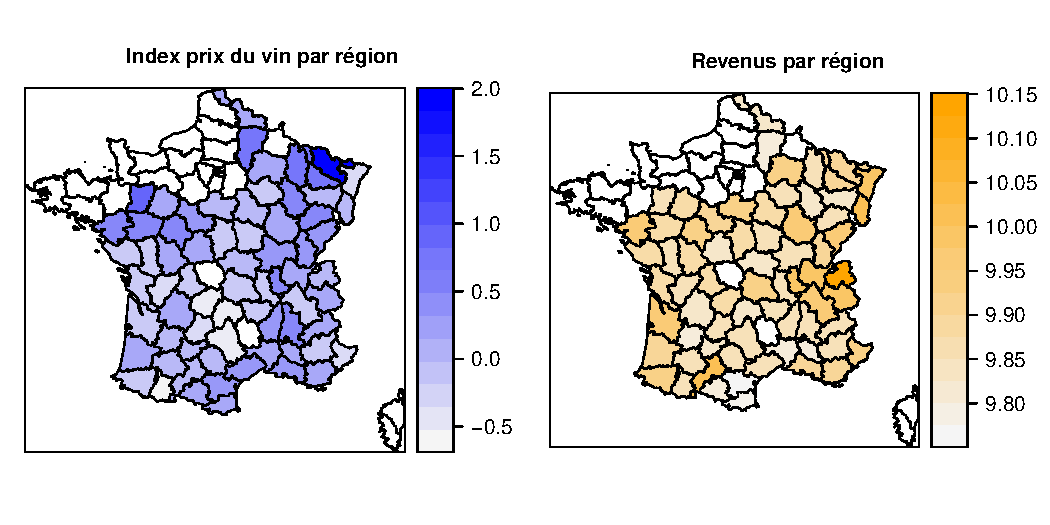
\includegraphics{note2pres_files/figure-latex/unnamed-chunk-17-1} 

}

\caption{Les quantité du vin non-IG moyennes par département}\label{fig:unnamed-chunk-17}
\end{figure}

\FloatBarrier

Puis, nous observons le comportement du reste des variables (les
représentations graphiques sont groupés dans l'annexe A1). L'indice des
prix se comporte pratiquement comme la quantité de vin produite, car cet
indice fut construit par l'intermédiaire de cette variable. Les autres
moyennes ne semblent pas avoir des structures corrélées dans l'espace au
niveau de la France. Dans notre analyse nous nous laissons la liberté
d'ignorer les effets possibles d'autocorrélation spatiale dans nos
données. En effet, au moment de la construction de notre base de
données, nous avons ignoré les départements ne produisant pas de vin
simple. Mais, ils peuvent quand même jouer un rôle si nous prenions en
compte la structure spatiale de nos données.

\hypertarget{etude-de-la-variance}{%
\subsection{Etude de la variance}\label{etude-de-la-variance}}

Passons maintenant, à l'étude de la variance. Nous allons décortiquer la
variance par type (between et within) afin d'obtenir une idée sur le
choix préférable de la dimension d'agrégation de nos données, car il se
peut que la théorie ne corresponde pas à la réalité (ex: nous faisons
face aux effets fixes par année et non par département).

Le tableau suivant regroupe les statistiques déscriptives essentielles :

\begin{itemize}
\tightlist
\item
  Moyennes
\item
  Variance sur l'échantillon complet
\item
  Variance \emph{between}
\item
  Variance \emph{within}
\end{itemize}

\FloatBarrier

\begin{table}[!htbp] \centering 
  \caption{Etude de la variance} 
  \label{} 
\begin{tabular}{@{\extracolsep{5pt}} ccccc} 
\\[-1.8ex]\hline 
\hline \\[-1.8ex] 
 & Mean & Overall & Between & Within \\ 
\hline \\[-1.8ex] 
Index prix & $1.431$ & $1.339$ & $1.012$ & $0.883$ \\ 
Index pesticides & $1.257$ & $0.483$ & $0.335$ & $0.350$ \\ 
Surface & $4.892$ & $1.986$ & $1.955$ & $0.410$ \\ 
Revenus & $9.891$ & $0.061$ & $0.061$ & $0.011$ \\ 
Temps & $3$ & $1.416$ & $0$ & $1.416$ \\ 
\hline \\[-1.8ex] 
\end{tabular} 
\end{table}

\FloatBarrier

Il est facile de remarquer que la variance \emph{between} est plus
grande que la variance \emph{within}. Cela nous amène à l'idée qu'il
faut utiliser un modèle qui permettra d'estimer et de corriger ces
inégalités entre les individus, car nous sommes plus interessés par des
effets individuels moyens (les effets moyens pour tous les
départements). Cela est complètement conforme à l'hypothèse que l'on a
exprimé lors de la formalisation du modèle économique théorique.

De plus, il est intéressant d'observer les résultats obtenus pour le
test de Chow comparant le modèle complet (\emph{pooled model}) contre
les modèles aux effets fixes et aléatoires. Le tableau suivant regroupe
les p-valeurs de ce test pour les différents modèles univariées.

\FloatBarrier

\begin{table}[!htbp] \centering 
  \caption{Pooling-test de Chow, p-valeurs} 
  \label{} 
\begin{tabular}{@{\extracolsep{5pt}} ccc} 
\\[-1.8ex]\hline 
\hline \\[-1.8ex] 
 & Random & Fixed \\ 
\hline \\[-1.8ex] 
Index prix & $0$ & $0$ \\ 
Index pesticides & $0.354$ & $0.294$ \\ 
Surface & $0$ & $0.0001$ \\ 
Revenus & $0.297$ & $0.247$ \\ 
\hline \\[-1.8ex] 
\end{tabular} 
\end{table}

\FloatBarrier

A part le cas de la surface nous ne pouvons pas rejeter l'hypothèse
nulle, spécifiant que les individus ont des effets identiques pour toute
la population.

\hypertarget{letude-des-types-deffets}{%
\subsection{L'étude des types d'effets}\label{letude-des-types-deffets}}

Nous avons déjà vu, qu'il est fortement probable que nous faisions face
à un modèle à effets fixes individuelles. Il faut quand même le
justifier. Pour faire cela, nous allons effectuer le test du
multiplicateur de Lagrange sur la nature des effets (individuels,
temporels ou en double dimension). Selon les résultats des tests il est
difficile de choisir arbitrairement un type d'effet. Il est évident que
nous avons des effets fixes au niveau individuel ou des effets fixes en
double dimension pour toutes les variables.

\FloatBarrier

\begin{table}[!htbp] \centering 
  \caption{p-valeurs de Lagrange multiplier test} 
  \label{} 
\begin{tabular}{@{\extracolsep{5pt}} cccc} 
\\[-1.8ex]\hline 
\hline \\[-1.8ex] 
 & Individual & Time & Twoways \\ 
\hline \\[-1.8ex] 
Index prix & $0$ & $0.256$ & $0$ \\ 
Index pesticides & $0$ & $0.229$ & $0$ \\ 
Surface & $0$ & $0.030$ & $0$ \\ 
Revenus & $0$ & $0.248$ & $0$ \\ 
\hline \\[-1.8ex] 
\end{tabular} 
\end{table}

\FloatBarrier

Selon les résultats obtenus, ainsi que les évidences théoriques des
études antérieurs nous décidons de ne garder que les effets fixes au
niveau individuel afin de faciliter l'analyse.

\hypertarget{lanalyse-de-la-correlation}{%
\subsection{L'analyse de la
corrélation}\label{lanalyse-de-la-correlation}}

Dans le tableau A2.2 des annexes nous présentons les corrélations des
variables après la correction pour les effets fixes individuels (nous
effectuons la transformation \emph{within} sur nos données en
soustrayant les moyennes individuelles pour l'ensemble des variables).
Dans les annexes, nous proposons également un tableau de corrélation
pour les données non-transformées (A2.1), ce qui permet d'observer les
inégalités et une pauvre répresentativitée des liens entres les
variables pour les données initiales. Il est facile à remarquer la
corrélation des ordres inférieurs à 0.1 pour toutes les variables sauf
les intéractions entre la surface cultivé et la quantité de vin offerte,
ce qui explique pourquoi nous n'avons pas le choix et devons passer à la
forme \emph{within}.

En ce qui concerne les données \emph{within}, particulierement nous
pouvons remarquer une forte corrélation entre la quantité offerte et le
prix d'équilibre. Egalement nous observons une corrélation positive
suffisamment significative (supérieure en grandeur de 0.2) entre la
surface cultivé et la quantité du vin simple sur le marché, aussi bien
qu'entre les revenus et l'indice d'utilisation des pesticides (ce qui
est probablement juste une coïncidence). Finalement, nous remarquons une
corrélation négative entre la surface cultivée et l'indice d'utilisation
des pesticides, ce qui est tout à fait naturel.

\hypertarget{modelisation}{%
\section{6. Modèlisation}\label{modelisation}}

\noindent

\rule[0.5ex]{\linewidth}{1pt}

\textcolor{red}{Ajouter des liens avec des études méthodologiques precedents.}

\noindent

\rule[0.5ex]{\linewidth}{1pt}

Cette partie du travail abordera la formulation économétrique de notre
problème. Nous allons débuter par la présentation des notions théoriques
utilisées dans ce travail, suivis par la formalisation économétrique du
modèle théorique que nous avons spécifié dans la séction 5. Après, nous
expliquerons la stratégie d'identification utilisée.

\hypertarget{presentation-de-la-methodologie}{%
\subsection{Presentation de la
méthodologie}\label{presentation-de-la-methodologie}}

L'AIDS (\emph{almost ideal demand system}) et les autres modèles de
demande cités dans la littérature ont de nombreuses lacunes qui les
rendent impropres pour l'estimation du marché du vin, selon Cembalo,
Caracciolo, and Pomarici (2014). Dans notre étude nous allons, tout de
même, utiliser une approche similaire à ce modèle là, sous des
suppositions restrictives.

Ce modèle nous permettra de simuler l'équilibre sur le marché du vin,
prenant ainsi en compte la plupart des facteurs incitant les producteurs
de vin à utiliser les pesticides.

\hypertarget{modele-econometrique}{%
\subsection{Modèle économétrique}\label{modele-econometrique}}

Dans cette section, nous allons présenter un par un nos modèles
économétriques correspondant chacun à un des trois cadres théoriques
possibles. Tous les modèles visent à estimer les effets moyens pour tous
les départements sous des hypothèses différentes de fonctionnement de
marché. Dans tous les cas, l'agrégation des effets au niveau national
(ou au niveau des groupes) nous permet de réduire les biais eventuels,
liés à la mauvaise spécification du modèle.

Pour le cadre où nous n'observons pas les intéractions entre la demande
et l'offre sur le marché (M1). Nous estimons un modèle simple. Nous
écrivons notre modèle sous la forme suivante :

\begin{equation*}
  qo_{i,t} = a_1 + b Po_{i,t} + c X_{i,t} + u_{i,t}
\end{equation*}

A ce point nous avons un choix : soit nous supposons que les
agriculteurs sont des preneurs de prix, ce qui nous permet de traiter le
prix comme une variable exogène; soit nous devrions construire un
estimateur de variables instrumentales afin de traiter l'endogénéité
éventuelle de l'indice des prix. Evidement le premier cas est le plus
simple, mais pour justifier l'utilisation de cette méthode nous devrions
effectuer des tests d'endogénéité de prix. Le deuxième cas est beaucoup
plus réaliste, puisque les viticulteurs sont rarement preneurs de prix
et l'offre aussi joue son rôle sur l'équilibre du marché.

Dans la dernière situation nous utilisons les idées de MacKay and Miller
(2018), supposant que les variables déterminant la demande sont des
instruments fiables pour la prédiction des variables endogènes dans
l'équation d'offre (bien que dans notre cas nous ignorons les effets des
intéractions entre l'offre et la demande). Particulièremnt ici, nous
pourrions utiliser les données sur les revenus afin d'instrumenter le
niveau des prix (l'indice des prix du vin).

Passons maintenant au modèle plus complexe (M2), basé sur l'hypothèse
que la demande influence l'offre, affectant également l'utilisation des
pesticides par les agriculteurs. Nous pouvons réécrire notre système
d'équations dans ce cas sous la forme suivante :

\begin{align*}
  qo_{i,t} & = a_1 + b Po_{i,t} + c X_{i,t} + u_{i,t} \\ 
  qd_{i,t} & = \alpha_{i} + \beta Pd_{i,t} + \gamma Z_{i,t} + \epsilon_{i,t}  \\
\end{align*}

Nous posons que l'offre et la demande sont egaux au niveau de chaque
département : \(qd_{i,t} = qo_{i,t}\). C'est-à-dire que l'offre interne
du département vise à satisfaire la demande interne du même département.

En termes d'agrégation ex-post des effets estimés, nous sommes sensés
tomber sur l'équilibre au niveau du marché national. En d'autre mots, le
système (qui implique : \(Qd = Qo\)) :

\begin{equation*}
  qd_{i,t} = qo_{i,t}
\end{equation*}

Au point d'équilibre nous rencontrons également l'égalité des prix :

\begin{equation*}
  Po_{1,t} = Pd_{1,t}
\end{equation*}

De cette façon nous obtenons un système d'équations. En simplifiant
l'écriture nous pouvons la représenter sous la forme suivante :

\begin{align*}
  q_{i,t} & = \alpha_{i} + \beta P_{i,t} + \gamma Z_{i,t} + \epsilon_{i,t} \\
  q_{i,t} & = a_i + b P_{i,t} + c X_{i,t} + u_{i,t}
\end{align*}

Et finalement, nous pouvons estimer les deux modèles (M1 et M2) en
regroupant les départements par leurs caractéristiques. Appelons ces
modèles M3.1 et M3.2 respectivement.

Le premier prenant la forme :

\begin{align*}
  qo_{i,t} & = a_1 + b Po_{i,t} + c X_{i,t} + u_{i,t} \\ 
\end{align*}

Tandis que le dernier :

\begin{align*}
  q_{i_{c},t} & = \alpha_{i_{c}} + \beta P_{i_{c},t} + \gamma Z_{i_{c},t} + \epsilon_{i_{c},t} \\
  q_{i_{c},t} & = a_i + b P_{i_{c},t} + c X_{i_{c},t} + u_{i_{c},t}
\end{align*}

Avec \(c\) décrivant l'appartenance du département à un des clusters.

Pour finir cette partie, nous avons à notre disposition plusieurs
chemins différents pour traiter ce modèle du point de vue économétrique.
Le plus simple est d'estimer l'effet des pesticides sur l'offre de vin
en ignorant les impacts du comportement des consommaterus sur les
producteurs. Cette méthode implique une estimation par OLS simples (ou
IV-OLS, lesquels introduisent la notion d'endogénéité des prix). De
l'autre coté, nous pouvons utiliser les triples moindre carrés (nous
devrions comparer les résultats obtenus avec un système d' équations
non-réliées, éstimé par 2SLS afin de traiter l'endogenèité), qui nous
permettront d'obtenir des résultats identiques aux résultats
d'estimations des équations structurelles sous l'hypothèse de
l'intéraction entre l'offre et la demande. Cette méthode offre la
possibilité d'estimer le système d'équations avec plusieurs variables
endogènes en prenant en compte les deux coté du marché, à la fois.
Finalement, si on trouve qu'il existe une hétérogénéité entre les
départements en termes d'équilibre interne, nous pourrions réestimer les
modèles en clusterisant nos \emph{individus} (départements) par des
classes différentes selon leurs attributs, pour estimer les equations
par cluster.

\hypertarget{hypotheses-sur-les-resultats}{%
\subsection{Hypothèses sur les
résultats}\label{hypotheses-sur-les-resultats}}

Nous attendons que l'estimateur de 3SLS, qui permet de capter les effets
de corrélations entre les équations en présence de plusieures variables
exogènes nous permettra d'obtenir des estimations plus fiables. Cette
méthode nous permet à depasser le biais de simultanéité qui apparaît
dans le cas d'estimation des systèmes d'équations liés (dans notre cas
nous étudions les effets des pesticides sur l'offre et production du vin
simple sous l'hypothèse de présence des effets du marché). L'estimateur
pareil donne des résultats similaires à l'estimateur de ILS
(\emph{indirect least squares}). De plus, sa version iterée (qui
converge à des résultats similaires à ceux obtenus par l'éstimation avec
maximum de vraisamblance) donne des résultats avec la variance la plus
faible.

Les propriétés de cet estimateur sont :

\begin{itemize}
\tightlist
\item
  Consistence ;
\item
  Efficience (asymptotique) ;
\item
  La distributions pour les estimateurs suit une loi normale seulement
  dans des grands échantillons.
\end{itemize}

Dès le debut nous envisagions que cet estimateur ne reflètera pas la
nature du marché. C'est pourquoi nous, dans ce travail, testons
plusieurs modèles.

Parmi les inconvénients éventuels, on a également la faible
représentation des effets hetérogènes entre les départements par le
modèle. Nous estimons seulement les effets moyens et ainsi nous ignorons
les différences des élasticités pour des départements différents.
Hereusement ce problème peut être rémédié par l'introduction des
clusters, regroupant des départements ayant des comportements
similaires.

Finalement, il existe des effets que l'on ignore complètement, mais qui
risquent d'intervenir. Par exemple, nous ignorons la présence
d'autocorrélation spatiale et/ou temporelle dans notre modèle.
Egalement, un nombre probablement insuffisant de facteurs est utilisé
dans ce modèle, ce qui augmente le risque du biais des variables omises
dans nos estimations.

\hypertarget{resultats-des-estimations}{%
\section{7. Résultats des estimations}\label{resultats-des-estimations}}

Dans cette section nous allons présenter les résultats économétriques
pour les différents modèles et les comparer.

Nous estimons un ensemble de modèles différents possibles afin de
pouvoir choisir la méthode la plus raisonnable. Les modèles suivants
sont traités séparement :

\begin{itemize}
\tightlist
\item
  M1 : modèle simple sans intéraction entre l'offre et la demande ;
\item
  M2 : modèle complexe visant à intégrer les intéractions entre l'offre
  et la demande en présence de variables éndogènes ;
\item
  M3 : les modèles sur les données clustérisées (M3.1 et M3.2
  respectivement pour les deux cas précédents).
\end{itemize}

\hypertarget{m1-les-resultats-en-absence-dinteractions}{%
\subsection{M1 : Les résultats en absence
d'intéractions}\label{m1-les-resultats-en-absence-dinteractions}}

Dans le cas des modèles sans intéractions avec la demande, nous pouvons
séparer deux cas différents. Le premier, le plus simple, se base sur
l'hypothèse, que les prix des vins simples sont imposés aux agriculteurs
par les consomateurs (ou, ce qui est beaucoup plus probable, par des
grandes enseignes ayant un pouvoir de négociation significatif). Cela
implique que nous pouvons considèrer les prix comme exogènes dans notre
modèlisation d'offre et par conséquent estimer notre modèle par des MCO
(OLS - \emph{ordinary least squares}) simples. En ce qui concerne le
deuxième cas, nous posons que les prix dans l'equation d'offre sont
endogènes. C'est-à-dire, les agriculteurs affectent les prix par leur
niveau de production et par les quantités émises sur le marché final.
Afin de traiter ce problème d'endogénéité nous pouvons utiliser la
méthode des variables instrumentales (IV-OLS). Mais quels instruments
choisir ? Sur ce point nous nous référons au travail de MacKay and
Miller (2018) (et plus particulierement le travail fondateur de Hausman
(1996)), où les auteurs démontrent que les instrument d'offre choisis
parmis les régresseurs de l'équation de la demande sont des instruments
suffisament pertinents. Dans notre cas nous pouvons instrumenter les
prix par les revenus dans les départements étudiés, ce qui est conforme
à la théorie économique, car le niveau des prix doit être corrélé avec
le revenu réel.

Neanmoins, nous allons encore vérifier la validité de cet instrument et
du modèle résultant. Par exemple, bien que notre supposition sur
l'instrument rentre parfaitement dans le cadre théorique, nous
n'observons qu'une faible corrélation entre l'indice des prix et les
revenus (voir l'annexe A2.2). Les revenus ont la pus petite corrélation
avec la variable explicative quand même.

Les résultats pour les deux modèles sont présentés dans le tableau
ci-aprés :

\FloatBarrier

\begin{table}[!htbp]
\begin{center}
\begin{tabular}{l c c }
\hline
 & OLS & IV-OLS \\
\hline
IP           & $0.30^{***}$  & $-0.28$      \\
             & $(0.02)$      & $(0.25)$     \\
Surface      & $0.23^{***}$  & $0.47^{***}$ \\
             & $(0.04)$      & $(0.13)$     \\
I pésticides & $-0.16^{***}$ & $-0.11$      \\
             & $(0.05)$      & $(0.09)$     \\
\hline
R$^2$        & 0.52          & -0.87        \\
Adj. R$^2$   & 0.52          & -0.89        \\
Num. obs.    & 345           & 345          \\
RMSE         & 0.29          & 0.58         \\
\hline
\multicolumn{3}{l}{\scriptsize{$^{***}p<0.001$, $^{**}p<0.01$, $^*p<0.05$}}
\end{tabular}
\caption{Modèles économétriques, variable dépendante - la quantité du vin vendu (en log)}
\label{table : ols et ivols}
\end{center}
\end{table}

\FloatBarrier

Avant de commenter les effets estimés, nous devons supposer que le
modèle en présence d'endogénéité n'est pas correcte (les estimateurs
obtenus sont biaisé et loins de la réalité). D'abord, les instruments
utilisé pour l'estimer sont asssez faibles et donne pas des résultats
pertinents. De plus, à partir des résultats du test de Wu-Haussman nous
pouvons conclure qui nous indique que les estimateurs OLS et IV-OLS sont
identiquement consistent et que nous n'avons pas des raisons pour
utiliser l'estimateurs de IV-OLS (dans cette situation les résultats
obtenus par OLS sont plus efficaces). Les résultats de ces tests sont
regrouppés dans l'annexe X.

Toutefois, les résultats obtenus par l'estimateur de OLS risquent d'être
également biaisés. Dans l'annexe X nous pouvons voir que Shapiro-Wilk
test rejette la normalité des résidus de notre modèle (annexe B4), bien
que la fonction de répartition partielle a une forme proche à normale
(annexe B1). Nous risquons également d'avoir des biais dans la variance
des estimateurs, car selon le test de Bartlett sur l'heteroscedacité
nous réjétons l'hypothèse de l'homoscedacité des résidus (annexe B3). Au
moins dans ce cas nous n'avons pas des problèmes avec l'autocorrelation
(les résultats du test de Durbin-Watson sont grouppé dans l'annexe B2),
ce qui peut s'expliquer par utilisation des données temporelles en série
trop courte pour y pouvoir detecter l'autocorrelation. Les résidus
également ne sont pas correlé avec des variables explicatives, mais ont
oune correlation forte avec la variable dependante, ce qui nous indique
sur la misspécification possible dans notre modèle (annexe B1).
L'explication la plus probable à ce problème est qu'on n'étudie pas
suffisament d'effets dans notre modèle et rencontrons par suite le biais
de variable omise. Le graphique des résidus nous montre en même temps la
nature quasi-aléatoire des résidus.

Maintenant, passons au résultats obtenus. L'indexe des prix a une faible
effet positive sur l'équilibre du marché. Néanmoins il n'est pas trop
sensible de commenter ces effets plus précisement, car nous n'avons
toujour pas une évidence forte sur sa exogénité. La surface dediée au
vins simples a également un effet positive sur la quantité du vin simple
vendu, ce qui est toutà fait naturelle, vu que c'est le facteur
principal de production du vin. Finalement, nous passons à l'effet le
plus interessant dans le contexte de notre étude. Nous rappelons à notre
lecteur que c'est exactement cet effet, l'effet des pésticides sur le
marché du vin, qu'on vise à estimer. Conformement aux études precedents
nous découvrons que les pésticides ont un impact négative sur l'offre du
vin simple, ce qui s'explique par leur nature d'utilisation.
C'est-à-dire, nous obtenons une confirmation que les pésticides sont
utilisés pour minimiser les pertes par les agriculteurs.
Particulierement dans le cadre du modèle estimé, l'effet moyen pour
l'ensemble des départements est qu'une augmentation de 1\% d'utilisation
des pésticides est une reponse des agriculteurs à des pértes et de la
baisse de l'offre d'au moint de 0.0016\%, toutes choses égales par
ailleurs. Les résultats en termes numeriques sont assez ambigus, car
nous faisons face à des nombreux problèmes dans la spécification du
modèle, quand même nous pouvons constater un effet de minimisation des
pertes dans l'utilisation des pésticides.\\
Cette nature révele des implications importantes en termes de traitement
futur du problème d'utilisation excessif des pésticicdes dans la
viticulture.

\hypertarget{m2-les-resultats-dans-le-cas-des-effets-du-marche-presents}{%
\subsection{M2 : Les résultats dans le cas des effets du marché
presents}\label{m2-les-resultats-dans-le-cas-des-effets-du-marche-presents}}

Dans cette séction nous allons étudier le modèle sous l'hypothèse de
présence des effets de la conjoncture sur les décisions des
agriculteurs. Identiquement au cadre précedent nous avons deux choix
possibles. D'abord, sous l'hypothèse d'endogénéité des prix nous povons
estimer le modèle par le méthode de 3SLS, en introduisant dans notre
modèle à la fois l'endogénéité des prix pour l'offre et la demande et la
correlation entre les résidus de ces deux équations décrivant le
comportement des agents du marché. Deuxiemement, nous avons la
possibilité d'imposer l'exogeneité des prix dans nos équations, ce qui
peut être les cas si les enseignes rachetant le vin des agriculteurs
sont des preneurs des prix du consommateur final. Nous allons comparér
des résultats des plusieurs modèles afin de verifier sa validité.

Le prémier modèle éstimé par les 3SLS est complexe et nous risquons
d'obtenir des résultats biaisé suite à des misspécification eventuelles.
Afin de contracter la variance des estimateurs les rendant plus
efficaces nous pouvons impliquer la procedre i3SLS (\emph{iterated three
step least squares}). Cette méthode nous donne des résultats similaire à
ceux obtenus par FIML (\emph{full information maximum likelihood}).
Quand même l'utilisations des procedures itératives ne semble pas donner
une diminution dans les variances des estimateurs significative (annexe
C1).

Nous pouvons également comparer les résultats obtenus par 3SLS avec le
modèle en absence des intéractions (sous l'hypothèse que les résidus des
deux équations ont une correlation nulle) éstimé par 2SLS (\emph{two
step least squares}). Dans ce cas, les regresseurs endogenes de la
demande sont instrumentés tout comme décrit dans Wooldridge (2005). Ce
méthode donne des résultats équivalents à ILS (\emph{indirect least
squares}), une téchnique utilisé pour estimer les systémés des
équations.

Dans le deuxieme cas nous réjetons l'hypothèse de l'endogénéité des prix
pour le marché du vins simple, en supposant qu'il est dicté par le
consommateurs final à les acteurs en amont (le distributeur qui rachete
le vin d'agriculteur). Cela nous amène à implementer le méthode SUR
(\emph{seamingly unrelated equations}) afin d'introduire la correlation
entre les résidus dans notre modèle du marché tout en ignorant
l'endogénéité des prix.

Les résultats pour les deux modèles sont régrouppé sous format d'un
tableau ci-dessous (``D'' désigne les coefficients de l'équation de la
demande et ``O'' de l'équation de l'offre, qui nous interesse) :

\FloatBarrier

\begin{table}[!htbp]
\begin{center}
\begin{tabular}{l c c }
\hline
 & SUR & 3SLS \\
\hline
D : IP              & $0.32^{***}$ & $0.79^{***}$   \\
                    & $(0.02)$     & $(0.15)$       \\
D : Revenu          & $-1.10$      & $-13.07^{***}$ \\
                    & $(0.66)$     & $(2.76)$       \\
O : IP              & $0.32^{***}$ & $-0.25$        \\
                    & $(0.02)$     & $(0.25)$       \\
O : Surface         & $0.03$       & $0.45^{***}$   \\
                    & $(0.02)$     & $(0.13)$       \\
O : I pésticides    & $-0.02$      & $-0.17^{*}$    \\
                    & $(0.02)$     & $(0.08)$       \\
\hline
Demande: R$^2$      & 0.46         & -0.41          \\
Offre: R$^2$        & 0.46         & -0.74          \\
Demande: Adj. R$^2$ & 0.45         & -0.42          \\
Offre: Adj. R$^2$   & 0.46         & -0.75          \\
Num. obs. (total)   & 690          & 690            \\
\hline
\multicolumn{3}{l}{\scriptsize{$^{***}p<0.001$, $^{**}p<0.01$, $^*p<0.05$}}
\end{tabular}
\caption{Modèles économétriques, variable dépendante - la quantité du vin vendu (en log)}
\label{table : sur et 3sls}
\end{center}
\end{table}

\FloatBarrier

Les résultats obtenus pour le cadre avec les prix endogènes
(l'estimation par 3SLS) donne forcement des résultats biaisé, car comme
nous avons vu dans la séctions précedente nous ne dispososns pas
d'instruments suffisament forts pour instrumenter l'index des prix. Cela
se confirme par la nonsignificativité des indices des prix estimé par
l'approche des variables instrumentalles. Ces effets sont négatives
non-differents de zero, ce qui n'est pas normal pour un bien n'étant le
bien de Giffen (bien que nous pouvons arbitrer que le vin le plus ismple
pourrais se comporter d'une telle façon, car c'est un des produits
alimentaires les plus basiques). Des autres tests nous confirment la
misspécification de ctte modèle : les résidus sont parfaitment correlé
avec les valeurs de variable dépendante et les prédictions, ce qui est
evident des graphiques dans les annexe C2; une forte hétereroscedacité,
qui cette fois est apparente sur les graphiques (annexes C2 et C5), etc.
Quand même les tests de spécification ne donne pas aucune indication de
misspécification du modèle 3SLS par rapport au modèle 2SLS, ce qui nous
rassure dans notre supposition que nous n'utilisaons pas suffisament des
variables explicatives dans notre modèle pour utiliser ces approches
économétriqes.

Tout de même, nous obtenons des résultats proches à ceux obtenus par OLS
simples dans la séction precedente (\(-0.16\) contre \(-0.17\)). Cela
confirme notre hypothèse sur le rôle joué par les pésticides dans la
propositions du vin simple sur le marché. Néanmoins, nous préferions de
ne pas utiliser ce modèle comme notre modèle de réference en futur à
cause de plusieurs sources des biais.

En ce qui concerne les résultats d'estimation par SUR, nous constatons
des effets sont presque idéntiques à ceux, obtenus par l'estimateur OLS
simple. Bien que dans ce cas les effets d'utilisation des pésticides
sont un peu plus accentués, avec un comportement des résidus plus
abnormaux.

\hypertarget{m3-les-resultats-pour-des-departements-grouppes}{%
\subsection{M3 : Les résultats pour des départements
grouppés}\label{m3-les-resultats-pour-des-departements-grouppes}}

Dans cette séction nous allons commencer par la présentation et la
comparaison des differentes téchniques pour la clustérisation de nos
données. Puis nous allons proceder avec un étude et la modèlisation des
données clustérisé. Nous suppososn que cet approche peut donner des
résultats significativement differents, car nous supposons une forte
héterogeneité dans le comportement des differents départements.

Le regrouppement des département dans les clusters par leurs
caractéristiques possiblement proches, doit nous permettre de traiter
les problèmes d'hétérogénéité possibles (nous pouvons observer des
traces de ces effets sur les graphiques dans l'annexe A2). Cela devra
permettre d'ameillorer les résultats des estimations en réduisant la
variance de nos estimateurs.

\hypertarget{clusterisation}{%
\subsubsection{Clusterisation}\label{clusterisation}}

Il existent plusieurs façons de séparer et clustériser les données.
Nous, dans notre travail, allons implementer la procedure \emph{k-means}
ou \emph{k-moyennes}. Cette procedure regrouppes les individus autours
des \emph{centres} (dont le nombre est \emph{k}) choisis par un
algorithme itérative. Cet algorithme itérative minimise la distance
inta-cluster. La qualité d'ajustement des clusters est evalué par le
paramétre WSS (\emph{within sum of squares}). C'est exactement ce
paramétre la qu'on va utiliser pour comparer les differents approches et
en choisir le plus approprié.

En ce qui concerne les differents méthodes de clustérisation, nous
pouvons les choisir en manipulant les données à l'entrée (les
\emph{inputs}) de cet algorithme. Plus précisement nous pouvons :

\begin{itemize}
\tightlist
\item
  Groupper les départements en utilisant les valeurs moyennes
  pluriannuelles de leurs caractéristiques (ce qui est idéntique aux
  données qu'on obtient lors de la transformation \emph{between});
\item
  Groupper nos individus en utilisant les variations des
  caractéristiques intra-annuelles (nous appliquons la transformation
  \emph{within} à nos données, puis nous trasformons nos données afin de
  conserver la dimention temporelle);
\item
  Utiliser l'information complete pour capter les évolutions aussi bien
  que les differences générales entre les département étudiés.
\end{itemize}

\hypertarget{between}{%
\paragraph{\texorpdfstring{\emph{Between}}{Between}}\label{between}}

Nous supposons que les départements ayant des valeurs moyennes
inter-annuelles proches, obtenus par la transformation \emph{between},
ont des caractéristiques proches, ainsi qu'un comportement presque
identique. La clusterisation est effectuée sur les données
\emph{between} pour l'ensemble des départements étudiés.

Les résultats des éstimations ainsi que les centres théoriques pour
\(k = 3\) se trouvent dans l'annexe D1.1.

\hypertarget{within}{%
\subsubsection{\texorpdfstring{\emph{Within}}{Within}}\label{within}}

Dans ce cas nous supposons que les départements ayant des tendances et
les évolutions de leurs caractéristiques identiques ont un comportement
qui ressamble. Plus, précisement, nous commençon par la transformation
des nos données en \emph{within}, ce qui implique qu'on substrait les
moyennes empiriques intra-annuelles pour toutes les caractéristiques.
Après, nous transformons les données créant pour chaque caractéristique
pour chaque année une variable séparée, ce qui permet de préserver la
dimention temporelle de nos données.

Les centres théoriques obtenus pour \(k = 3\) se trouvent dans l'annexe
D1.2.

\hypertarget{information-complete}{%
\subsubsection{Information complète}\label{information-complete}}

Dans le cas de l'information complète nous utilisons l'ensemble des
informations disponibles sur les individus afin de construire les
clusters. Nous utilisons l'approche similaire à celui utilisé dans le
cas de clusterisation \emph{within}, sauf que cette fois nous
n'effectuons pas la correction sur les valeurs moyennes intra-annuelles.

Les centres obtenus pour ce type des données sont presenté dans l'annexe
D1.3.

\hypertarget{comparaison-des-differentes-methodes}{%
\paragraph{Comparaison des differentes
méthodes}\label{comparaison-des-differentes-methodes}}

Afin de pouvoir comparer des valeurs differents de WSS (\emph{within
summ of squares}) nous allons visualiser la valeur dun indice :

\begin{equation*}
    WSS^{'} = \frac{WSS}{min(WSS)}
\end{equation*}

Ce qui nous permettra d'évaluer les écarts rélatives du WSS de sa valeur
minimale (pour nombre des clusters égal à 15). Le graphique suivant
démontre l'évaluation des valeurs de \(WSS^{'}\) pour les trois cas
differents de la définition des clusters :

\FloatBarrier

\begin{center}\includegraphics{note2pres_files/figure-latex/unnamed-chunk-40-1} \end{center}

\FloatBarrier

Nous pouvons observer que pour la transformation \emph{within} nous
observons la convergence la plus vite vers la valeure minimale de WSS.
Les deux autres approches au traitement et transformation des données
offrent une vitesse de convergence plus elevé, avec des valeurs
rélatives initiales également plus significatives.

Nous remarquons également que les valeurs optimales du nombre des
clusters dans les trois cas sont à peu près identiques (autours de 3 et
5), avec la meilleure approximation absolute est atteint pour les huit
cluster et reste rélativement inchangé après.

\hypertarget{m3.1-le-cadre-en-absence-des-interaction-avec-la-demande}{%
\subsubsection{M3.1 : Le cadre en absence des intéraction avec la
demande}\label{m3.1-le-cadre-en-absence-des-interaction-avec-la-demande}}

Nous commençons par la comparaison des résultats obtenus pour les
differents clusters avec les modèles de type OLS et IV-OLS.
C'est-à-dire, sous l'hypothèse de l'abcense des intérferences entre
l'offre et la demande.

Nous n'evaluons pas le système en introduisant les variables de grouppe
(dummy variables) car cela risque de biaiser les résultats à cause d'une
taille des grouppes differente. Afin d'éviter ce biais nous évaluons les
modèles par cluster.

Le tableau suivant regrouppe les 6 modèles éstimés (3 clusters avec 2
modèles par cluster, le nombre du cluster étant affiché après \emph{c}
dans le tableau) :

\FloatBarrier

\begin{table}[!htbp]
\begin{center}
\begin{tabular}{l c c c c c c }
\hline
 & OLS c1 & IV-OLS c1 & OLS c2 & IV-OLS c2 & OLS c3 & IV-OLS c3 \\
\hline
IP           & $0.51^{***}$ & $0.22^{*}$  & $0.15$   & $0.15$   & $0.69^{***}$  & $4.36$   \\
             & $(0.02)$     & $(0.10)$    & $(0.04)$ & $(0.04)$ & $(0.03)$      & $(4.60)$ \\
Surface      & $0.09^{*}$   & $0.19^{**}$ & $-0.54$  & $-0.59$  & $0.19^{***}$  & $-0.69$  \\
             & $(0.04)$     & $(0.07)$    & $(0.58)$ & $(0.58)$ & $(0.04)$      & $(1.14)$ \\
I pésticides & $-0.11^{*}$  & $-0.01$     & $7.58$   & $7.73$   & $-0.16^{***}$ & $0.14$   \\
             & $(0.04)$     & $(0.07)$    & $(4.62)$ & $(4.65)$ & $(0.04)$      & $(0.52)$ \\
\hline
R$^2$        & 0.79         & 0.55        & 0.92     & 0.92     & 0.76          & -15.69   \\
Adj. R$^2$   & 0.78         & 0.54        & 0.80     & 0.80     & 0.76          & -15.95   \\
Num. obs.    & 145          & 145         & 5        & 5        & 195           & 195      \\
RMSE         & 0.14         & 0.21        & 0.39     & 0.39     & 0.23          & 1.96     \\
\hline
\multicolumn{7}{l}{\scriptsize{$^{***}p<0.001$, $^{**}p<0.01$, $^*p<0.05$}}
\end{tabular}
\caption{Modèles économétriques, variable dépendante - la quantité du vin vendu (en log)}
\label{table : ols et ivols clusters}
\end{center}
\end{table}

\FloatBarrier

Nous observons que un cluster réssort d'une façon abnormale ayant des
valeurs d'une magnitude excessive (c'est le département numéro 57 où
l'indice a une variation intra-annuelle abnormale, on peut le considérer
comme un outlier et ne pas le commenter). En ce qui concerne les deux
autres clusters, nous observons qu'un entre eux comprend les
départements se spécialisant dans la production des vins simples (avec
des effets des prix, de surface et d'utilisation des pésticides
accentuté). L'autre regroupe des département qui montrent des effets
moins réssortissants et evidents.

Les diagnostiques détaillés sont présentes dans l'annexe D2, où tous les
tests principaux sont présents. Les tests sur la validité des
éstimateurs IV sont les plus interessants et se trouvent dans l'annexe
D2.3, ou nous observons que les estimations par les variables
instrumentale n'est pas toujours valide dans notre cas. On ne peut pas
rejeter l'hypothèse des faibles instruments seulement pour un des
clusters, et le test de Wu-Haussman donne des résultats négatives pour
tous les clusters, nous indiquant que le modèle OLS est préferable.
Finalement, les résidus sont toujours non-normaux, bien que les résults
du test sont les méilleurs dans l'ensemble (annexe D2.2).

\hypertarget{m3.2-le-cadre-dinterference-avec-la-demande}{%
\subsubsection{M3.2 : Le cadre d'interference avec la
demande}\label{m3.2-le-cadre-dinterference-avec-la-demande}}

Dans cette partie nous utilisons l'approche identique à celui qu'on a
déjà implementé dans la partie M2. Nous supposons, que le marché
fonctionne en presence des liens entre l'offre et la demande. Les
résidus des deux équations dans ce cas sont correlés entre eux.

Identiquement à la section précedente nous régrouppons les résultats
d'estimation pour les 6 modèles (2 modèles par 3 clusters) sous la forme
d'un tableau.

\FloatBarrier

\begin{table}[!htbp]
\begin{center}
\begin{tabular}{l c c c c c c }
\hline
 & SUR c1 & 3SLS c1 & SUR c2 & 3SLS c2 & SUR c3 & 3SLS c3 \\
\hline
D : IP              & $0.52^{***}$ & $0.66^{***}$  & $0.12^{*}$ & $0.12^{*}$ & $0.73^{***}$  & $1.35^{***}$  \\
                    & $(0.02)$     & $(0.11)$      & $(0.03)$   & $(0.03)$   & $(0.03)$      & $(0.27)$      \\
D : Revenu          & $-0.86$      & $-6.68^{***}$ & $18.14$    & $18.43$    & $-4.87^{***}$ & $-10.08^{**}$ \\
                    & $(0.45)$     & $(1.95)$      & $(14.50)$  & $(14.62)$  & $(1.05)$      & $(3.51)$      \\
O : IP              & $0.51^{***}$ & $0.20^{*}$    & $0.16$     & $0.16^{*}$ & $0.72^{***}$  & $4.71$        \\
                    & $(0.02)$     & $(0.10)$      & $(0.04)$   & $(0.04)$   & $(0.03)$      & $(4.58)$      \\
O : Surface         & $0.01$       & $0.18^{*}$    & $-0.66$    & $-0.69$    & $0.05^{*}$    & $-0.68$       \\
                    & $(0.02)$     & $(0.07)$      & $(0.57)$   & $(0.58)$   & $(0.02)$      & $(1.14)$      \\
O : I pésticides    & $-0.01$      & $0.03$        & $4.97$     & $4.99$     & $-0.04$       & $0.43$        \\
                    & $(0.02)$     & $(0.07)$      & $(3.94)$   & $(3.93)$   & $(0.03)$      & $(0.38)$      \\
\hline
Demande: R$^2$      & 0.78         & 0.77          & 0.88       & 0.88       & 0.75          & 0.26          \\
Offre: R$^2$        & 0.77         & 0.52          & 0.89       & 0.89       & 0.73          & -19.07        \\
Demande: Adj. R$^2$ & 0.78         & 0.77          & 0.84       & 0.84       & 0.75          & 0.25          \\
Offre: Adj. R$^2$   & 0.77         & 0.52          & 0.78       & 0.78       & 0.73          & -19.27        \\
Num. obs. (total)   & 290          & 290           & 10         & 10         & 390           & 390           \\
\hline
\multicolumn{7}{l}{\scriptsize{$^{***}p<0.001$, $^{**}p<0.01$, $^*p<0.05$}}
\end{tabular}
\caption{Modèles économétriques, variable dépendante - la quantité du vin vendu (en log)}
\label{table : sur et 3sls clusters}
\end{center}
\end{table}

\FloatBarrier

Nous observons que les effets des pésticides sur la quantité marchande
du vin sont négligeables pour tous les clusters pour tous les modèles.
La validité de ces modèles laisse à désirer. D'abord, pour les modèles
supposant l'endogénéité des prix dans notre modèle nous avons des
instruments trop faibles, qui resultenet dans des modèles
non-efficients. De plus, l'introduction de l'hypothèse des liens entre
les deux cotés du marché (introduction de la correlation entre les
résidus) n'ameillore pas l'explicativité des modèles.

\hypertarget{avis-sur-lutilisation-des-clusters}{%
\subsubsection{Avis sur l'utilisation des
clusters}\label{avis-sur-lutilisation-des-clusters}}

En genéral les clusters n'ameilleurent pas les résumtats des
éstimations. Nous avons réussi à identifier un département trop
different du reste dans sa nature, mais en total cette méthode n'a
abouti à rien.

De plus, nous rétirons de ces tentatives d'ammeilloration de notre
modèle une evidence qu'il existent des département qui sont plus incliné
à la production du vin de table que le reste, ce qui est tout à fait
logique.

\hypertarget{conclusion}{%
\section{9. Conclusion}\label{conclusion}}

Nous avons étudié et comparé plusieurs modèles distincts qui visent à
apprécier les effets d'utilisation des pesticides sur l'offre de vin de
table. Nous constatons, que parmi tout ces modèles, le meilleur
estimateur des effets moyens par département est obtenu à travers un
simple modèle OLS en absence d'effets d'interaction avec la demande de
vin de table ou d'éndogénéité des prix. Ce fait est soutenu par les
hypothèses théoriques sur le fonctionnement du marché des vins simples
disponibles dans la littérature. Les agriculteurs proposant du vin
simples sont dans la plupart des cas preneurs des prix offerts par les
distributeurs, ce qui explique l'exogénéité des prix. Le même fait
explique l'absence des interactions entre l'offre et la demande, car les
grands enseignes achetes le vin simple sous conditions \emph{take or
leave} (ce qui n'est pas vrai pour les autres types du vin).

L'analyse des données clusterisées permet d'observer un degré
d'hétérogénéité relativement faible entre les départements. De plus, les
effets d'utilisation des pesticides sur l'offre de vin ne sont
clairement identifiables que pour un groupe spécifique d'entités
étudiées.

Les résultats obtenus dans cette étude confirment des résultats obtenus
par d'autres chercheurs, ainsi que les suppositions théoriques sur le
rôle des pesticides dans le commerce du vin. Plus precisement, les
pesticides sont utilisés par les viticulteurs pour minimiser les pertes
causées par les maladies, les fongicides\ldots{} etc. Nous captons ce
phénomène en estimant le modèle d'équilibre du marché du vin simple.

Nous devons également souligner que le modèle presenté dans ce travail
est loin de frôler la perfection absolue. Plusieurs problèmes restent
non-traité ou non-résolus. Parmi ces problèmes nous pouvons citer: un
faible nombre d'observations sur la dimention temporelle, la présence
d'heteroscedasticité dans les résidus, la non-normalité des résidus, des
variables omises, dess instruments faibles, etc. Toutefois, nous avons
reussi à capter la tendance principale dans le comportement de l'offre
face à l'utilisation des pesticides par les agriculteurs. Il peut donc
s'avérer interessant d'étudier ces aspects et de traiter ces problèmes
revelés dans de futures études.

Pour de futures recherches, nous conseillerons d'étudier directement
l'impact des pesticides sur la production et non sur l'équilibre du
marché parce que, comme nous avons pu le constater dans nos résultats,
la modélisation du marché via des équations simultanées ne nous permet
pas d'améliorer significativement nos estimateurs. Ceci constitue un
point important, étant donné le faible nombre de variables explicatives
sélectionnées et les défauts potentiels dans la spécification de notre
modèle, dans notre étude ces modèles se prouvent d'être innefficaces et
ne donne pas des résultats fiables.

\newpage

\hypertarget{annexes}{%
\section{Annexes}\label{annexes}}

\hypertarget{a-les-statistiques-descriptives}{%
\subsection{A Les statistiques
descriptives}\label{a-les-statistiques-descriptives}}

\hypertarget{a1-les-moyennes-par-departement}{%
\subsubsection{A1 Les moyennes par
département}\label{a1-les-moyennes-par-departement}}

\FloatBarrier

\begin{figure}[!htbp]

{\centering \includegraphics{note2pres_files/figure-latex/unnamed-chunk-50-1} 

}

\caption{Les valeurs moyennes par département}\label{fig:unnamed-chunk-50}
\end{figure}

\FloatBarrier

\newpage

\hypertarget{a2-letude-des-interdependances}{%
\subsubsection{A2 L'étude des
interdépendances}\label{a2-letude-des-interdependances}}

La premier de cet annexe combrend les résultats pour les données
telles-quelles, le deuxieme par contre integre les résultats pour les
données sous la trasformation \emph{within}.

\hypertarget{a2.1-information-complete}{%
\paragraph{A2.1 Information complète}\label{a2.1-information-complete}}

\FloatBarrier

\begin{figure}[!htbp]

{\centering 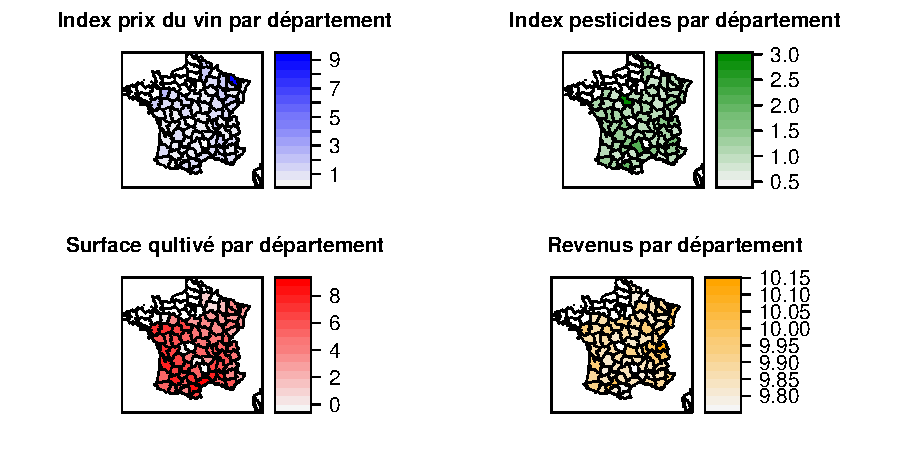
\includegraphics{note2pres_files/figure-latex/unnamed-chunk-51-1} 

}

\caption{L'étude bivarié}\label{fig:unnamed-chunk-51}
\end{figure}

\FloatBarrier

\FloatBarrier

\begin{table}[ht]
\centering
\begin{tabular}{l|rrrrrr}
  \hline
 & Quantité du vin & IP & Surface & Revenus & Index pésticides & Temps \\ 
  \hline
Quantité du vin & 1.00 & 0.02 & 0.96 & -0.03 & -0.07 & -0.04 \\ 
  IP & 0.02 & 1.00 & -0.05 & 0.01 & -0.06 & 0.11 \\ 
  Surface & 0.96 & -0.05 & 1.00 & -0.06 & -0.05 & -0.06 \\ 
  Revenus & -0.03 & 0.01 & -0.06 & 1.00 & -0.04 & 0.12 \\ 
  I pésticides & -0.07 & -0.06 & -0.05 & -0.04 & 1.00 & 0.30 \\ 
  Temps & -0.04 & 0.11 & -0.06 & 0.12 & 0.30 & 1.00 \\ 
   \hline
\end{tabular}
\caption{La correlation complete} 
\end{table}

\FloatBarrier

\newpage

\hypertarget{a2.2-transformation-within}{%
\paragraph{\texorpdfstring{A2.2 Transformation
\emph{within}}{A2.2 Transformation within}}\label{a2.2-transformation-within}}

Les rélations entre les variables mieux ressortent pour les données
transformées. Ce sont les données que nous intégrons dans nos modèles
économétriques.

\FloatBarrier

\begin{figure}[!htbp]

{\centering \includegraphics{note2pres_files/figure-latex/unnamed-chunk-54-1} 

}

\caption{Rélations bivariés dans le cas de transformation within}\label{fig:unnamed-chunk-54}
\end{figure}

\FloatBarrier

\FloatBarrier

\begin{table}[ht]
\centering
\begin{tabular}{l|rrrrrr}
  \hline
 & Quantité du vin & IP & Surface & Revenus & Index pésticides & Temps \\ 
  \hline
Quantité du vin & 1.00 & 0.67 & 0.37 & -0.16 & -0.18 & -0.20 \\ 
  IP & 0.67 & 1.00 & 0.19 & 0.11 & -0.01 & 0.16 \\ 
  Surface & 0.37 & 0.19 & 1.00 & -0.17 & -0.20 & -0.31 \\ 
  Revenus & -0.16 & 0.11 & -0.17 & 1.00 & 0.21 & 0.65 \\ 
  I pésticides & -0.18 & -0.01 & -0.20 & 0.21 & 1.00 & 0.41 \\ 
  Temps & -0.20 & 0.16 & -0.31 & 0.65 & 0.41 & 1.00 \\ 
   \hline
\end{tabular}
\caption{La correlation within} 
\end{table}

\FloatBarrier

\newpage

\hypertarget{b-analyse-des-resultats-du-cadre-m1}{%
\subsection{B Analyse des résultats du cadre
M1}\label{b-analyse-des-resultats-du-cadre-m1}}

\hypertarget{b1-le-compoertement-des-residus}{%
\subsubsection{B1 Le compoertement des
résidus}\label{b1-le-compoertement-des-residus}}

\FloatBarrier

\begin{table}[ht]
\centering
\begin{tabular}{l|rr}
  \hline
 & OLS & IV-OLS \\ 
  \hline
Vin & 0.69 & 0.88 \\ 
  IP & -0.00 & 0.85 \\ 
  Surface & 0.00 & 0.00 \\ 
  Revenus & -0.24 & 0.00 \\ 
  Pesticides & -0.00 & -0.00 \\ 
   \hline
\end{tabular}
\caption{Correlation des résidus} 
\end{table}

\FloatBarrier

\FloatBarrier

\begin{figure}[!htbp]

{\centering 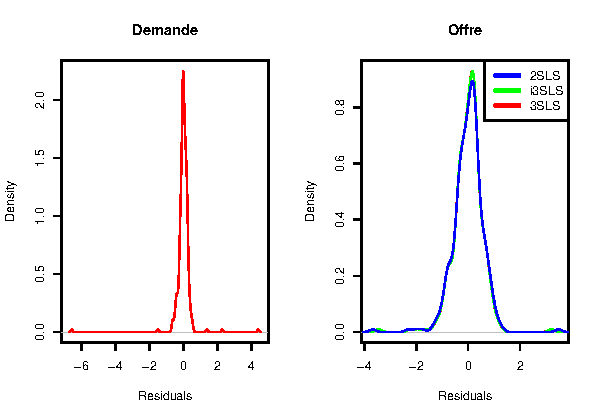
\includegraphics{note2pres_files/figure-latex/unnamed-chunk-59-1} 

}

\caption{Le comportement des résidus}\label{fig:unnamed-chunk-59}
\end{figure}

\FloatBarrier

\hypertarget{b2-lautocorrelation}{%
\subsubsection{B2 L'autocorrelation}\label{b2-lautocorrelation}}

\FloatBarrier

\begin{table}[!htbp] \centering 
  \caption{Les statistiques test de Durbin-Watson, t-stat} 
  \label{} 
\begin{tabular}{@{\extracolsep{5pt}} ccc} 
\\[-1.8ex]\hline 
\hline \\[-1.8ex] 
 & OLS & IV-OLS \\ 
\hline \\[-1.8ex] 
Equation d'offre & $0.627$ & $0.637$ \\ 
\hline \\[-1.8ex] 
\end{tabular} 
\end{table}

\FloatBarrier

\hypertarget{b3-test-de-lheteroskedacite}{%
\subsubsection{B3 Test de
l'hétéroskedacité}\label{b3-test-de-lheteroskedacite}}

\FloatBarrier

\begin{table}[!htbp] \centering 
  \caption{Les résultat du test de Bartlett sur l'heteroscedacité, p-valeur} 
  \label{} 
\begin{tabular}{@{\extracolsep{5pt}} ccc} 
\\[-1.8ex]\hline 
\hline \\[-1.8ex] 
 & OLS & IV-OLS \\ 
\hline \\[-1.8ex] 
Equation d'offre & $0$ & $0$ \\ 
\hline \\[-1.8ex] 
\end{tabular} 
\end{table}

\FloatBarrier

\hypertarget{b4-la-normalite-des-residus}{%
\subsubsection{B4 La normalité des
résidus}\label{b4-la-normalite-des-residus}}

\FloatBarrier

\FloatBarrier

\begin{table}[!htbp] \centering 
  \caption{Shapiro-Wilk test de normalité des résidus, p-valeur} 
  \label{} 
\begin{tabular}{@{\extracolsep{5pt}} ccc} 
\\[-1.8ex]\hline 
\hline \\[-1.8ex] 
 & OLS & IV-OLS \\ 
\hline \\[-1.8ex] 
Equation d'offre & $0$ & $0$ \\ 
\hline \\[-1.8ex] 
\end{tabular} 
\end{table}

\FloatBarrier

\hypertarget{b5-diagnostics-iv-ols}{%
\subsubsection{B5 Diagnostics IV-OLS}\label{b5-diagnostics-iv-ols}}

\FloatBarrier

\begin{table}[!htbp] \centering 
  \caption{Diagnostiques d'estimateur IV} 
  \label{} 
\begin{tabular}{@{\extracolsep{5pt}} ccccc} 
\\[-1.8ex]\hline 
\hline \\[-1.8ex] 
 & df1 & df2 & statistic & p-value \\ 
\hline \\[-1.8ex] 
Weak instruments & $2$ & $341$ & $3.645$ & $0.027$ \\ 
Wu-Hausman & $1$ & $341$ & $22.553$ & $0.00000$ \\ 
\hline \\[-1.8ex] 
\end{tabular} 
\end{table}

\FloatBarrier

\newpage

\hypertarget{c-analyse-des-resultats-m2}{%
\subsection{C Analyse des résultats
M2}\label{c-analyse-des-resultats-m2}}

\hypertarget{c1-comparaison-des-modeles-2sls-3sls-et-i3sls}{%
\subsubsection{C1 Comparaison des modèles 2SLS, 3SLS et
i3SLS}\label{c1-comparaison-des-modeles-2sls-3sls-et-i3sls}}

\FloatBarrier

\begin{table}[!htbp]
\begin{center}
\begin{tabular}{l c c c c }
\hline
 & SUR & 2SLS & 3SLS & i3SLS \\
\hline
D : IP              & $0.32^{***}$ & $0.79^{***}$   & $0.79^{***}$   & $0.79^{***}$   \\
                    & $(0.02)$     & $(0.15)$       & $(0.15)$       & $(0.15)$       \\
D : Revenu          & $-1.10$      & $-13.07^{***}$ & $-13.07^{***}$ & $-13.07^{***}$ \\
                    & $(0.66)$     & $(2.76)$       & $(2.76)$       & $(2.76)$       \\
O : IP              & $0.32^{***}$ & $-0.28$        & $-0.25$        & $-0.25$        \\
                    & $(0.02)$     & $(0.25)$       & $(0.25)$       & $(0.24)$       \\
O : Surface         & $0.03$       & $0.47^{***}$   & $0.45^{***}$   & $0.45^{***}$   \\
                    & $(0.02)$     & $(0.13)$       & $(0.13)$       & $(0.12)$       \\
O : I pésticides    & $-0.02$      & $-0.11$        & $-0.17^{*}$    & $-0.17^{*}$    \\
                    & $(0.02)$     & $(0.09)$       & $(0.08)$       & $(0.08)$       \\
\hline
Demande: R$^2$      & 0.46         & -0.41          & -0.41          & -0.41          \\
Offre: R$^2$        & 0.46         & -0.87          & -0.74          & -0.75          \\
Demande: Adj. R$^2$ & 0.45         & -0.42          & -0.42          & -0.42          \\
Offre: Adj. R$^2$   & 0.46         & -0.89          & -0.75          & -0.76          \\
Num. obs. (total)   & 690          & 690            & 690            & 690            \\
\hline
\multicolumn{5}{l}{\scriptsize{$^{***}p<0.001$, $^{**}p<0.01$, $^*p<0.05$}}
\end{tabular}
\caption{Modèles économétriques, variable dépendante - la quantité du vin vendu (en log)}
\label{table : sur, 2sls, 3sls and fiml}
\end{center}
\end{table}

\FloatBarrier

\newpage

\hypertarget{c2-independance-des-residus}{%
\subsubsection{C2 Indépendance des
résidus}\label{c2-independance-des-residus}}

\FloatBarrier

\begin{table}[ht]
\centering
\begin{tabular}{l|rrrrrrrr}
  \hline
 & SUR D & SUR O & 2SLS D & 2SLS O & 3SLS D & 3SLS O & i3SLS D & i3SLS O \\ 
  \hline
Vin & 0.75 & 0.75 & -0.13 & 0.88 & -0.13 & 0.88 & -0.13 & 0.88 \\ 
  IP & -0.00 & -0.00 & -0.80 & 0.85 & -0.80 & 0.84 & -0.80 & 0.84 \\ 
  Surface & 0.32 & 0.28 & 0.00 & 0.00 & 0.00 & -0.00 & 0.00 & -0.00 \\ 
  Revenus & -0.28 & -0.31 & 0.00 & -0.00 & 0.00 & 0.00 & 0.00 & 0.00 \\ 
  Pesticides & -0.23 & -0.20 & -0.08 & 0.00 & -0.08 & 0.03 & -0.08 & 0.03 \\ 
   \hline
\end{tabular}
\caption{Correlation des résidus} 
\end{table}

\FloatBarrier

\FloatBarrier

\begin{figure}[!htbp]

{\centering \includegraphics{note2pres_files/figure-latex/unnamed-chunk-72-1} 

}

\caption{Les résidus contre la variable prédite}\label{fig:unnamed-chunk-72}
\end{figure}

\FloatBarrier

\FloatBarrier

\begin{figure}[!htbp]

{\centering 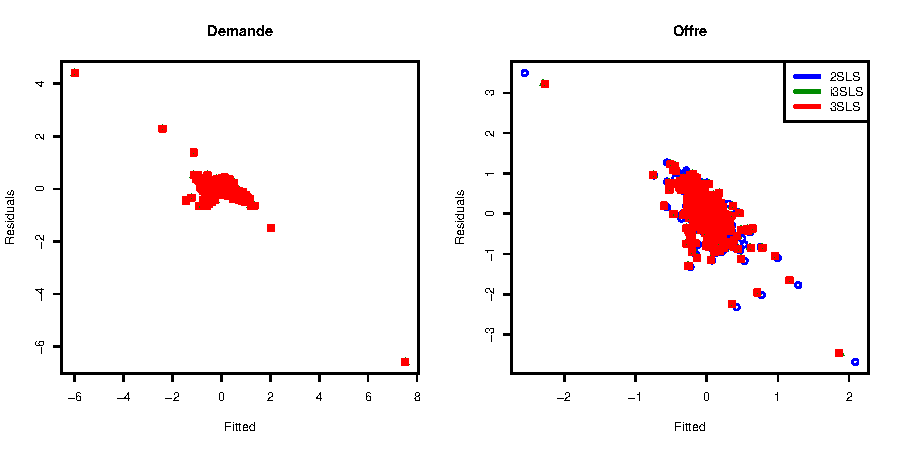
\includegraphics{note2pres_files/figure-latex/unnamed-chunk-73-1} 

}

\caption{Les résidus et les prédictions, le cas de SUR}\label{fig:unnamed-chunk-73}
\end{figure}

\FloatBarrier

\newpage

\hypertarget{c3-lautocorrelation}{%
\subsubsection{C3 L'autocorrelation}\label{c3-lautocorrelation}}

\FloatBarrier

\begin{table}[!htbp] \centering 
  \caption{Les resultats du test de Durbin-Watson, t-stat} 
  \label{} 
\begin{tabular}{@{\extracolsep{5pt}} ccccc} 
\\[-1.8ex]\hline 
\hline \\[-1.8ex] 
 & SUR & 2SLS & 3SLS & i3SLS \\ 
\hline \\[-1.8ex] 
Equation de demande & $0.687$ & $0.618$ & $0.618$ & $0.618$ \\ 
Equation d'offre & $0.683$ & $0.637$ & $0.638$ & $0.638$ \\ 
\hline \\[-1.8ex] 
\end{tabular} 
\end{table}

\FloatBarrier

\hypertarget{c4-test-de-lheteroscedasticite}{%
\subsubsection{C4 Test de
l'hétéroscedasticité}\label{c4-test-de-lheteroscedasticite}}

\FloatBarrier

\begin{table}[!htbp] \centering 
  \caption{Test de Bartlett sur l'heterockedacité, p-valeur} 
  \label{} 
\begin{tabular}{@{\extracolsep{5pt}} ccccc} 
\\[-1.8ex]\hline 
\hline \\[-1.8ex] 
 & SUR & 2SLS & 3SLS & i3SLS \\ 
\hline \\[-1.8ex] 
Equation de demande & $0$ & $0$ & $0$ & $0$ \\ 
Equation d'offre & $0$ & $0$ & $0$ & $0$ \\ 
\hline \\[-1.8ex] 
\end{tabular} 
\end{table}

\FloatBarrier

\hypertarget{c5-la-normalite-des-residus}{%
\subsubsection{C5 La normalité des
résidus}\label{c5-la-normalite-des-residus}}

\FloatBarrier

\FloatBarrier

\begin{table}[!htbp] \centering 
  \caption{Shapiro-Wilk test de normalité, p-valeur} 
  \label{} 
\begin{tabular}{@{\extracolsep{5pt}} ccccc} 
\\[-1.8ex]\hline 
\hline \\[-1.8ex] 
 & SUR & 2SLS & 3SLS & i3SLS \\ 
\hline \\[-1.8ex] 
Equation de demande & $0$ & $0$ & $0$ & $0$ \\ 
Equation d'offre & $0$ & $0$ & $0$ & $0$ \\ 
\hline \\[-1.8ex] 
\end{tabular} 
\end{table}

\FloatBarrier

\FloatBarrier

\begin{figure}[!htbp]

{\centering \includegraphics{note2pres_files/figure-latex/unnamed-chunk-80-1} 

}

\caption{Les PDF des résidus}\label{fig:unnamed-chunk-80}
\end{figure}

\FloatBarrier

\hypertarget{c6-comparaison-des-modeles}{%
\subsubsection{C6 Comparaison des
modèles}\label{c6-comparaison-des-modeles}}

\FloatBarrier

\FloatBarrier

\begin{table}[!htbp] \centering 
  \caption{Hausman 3SLS consistency test, p-valeur} 
  \label{} 
\begin{tabular}{@{\extracolsep{5pt}} ccc} 
\\[-1.8ex]\hline 
\hline \\[-1.8ex] 
 & Test & Resultats \\ 
\hline \\[-1.8ex] 
1 & 3SLS contre 2SLS & $1$ \\ 
2 & 3SLS contre SUR & $0$ \\ 
\hline \\[-1.8ex] 
\end{tabular} 
\end{table}

\FloatBarrier

\FloatBarrier

\begin{table}[ht]
\centering
\begin{tabular}{c|ccccc}
  \hline
 & \#Df & LogLik & Df & Chisq & Pr($>$Chisq) \\ 
  \hline
1 & 8 & 816.10 &  &  &  \\ 
  2 & 6 & -514.91 & -2 & 2662.02 & 0.0000 \\ 
  3 & 8 & -504.97 & 2 & 19.89 & 0.0000 \\ 
  4 & 8 & -505.66 & 0 & 1.38 & 0.0000 \\ 
   \hline
\end{tabular}
\caption{ML test de spécification} 
\end{table}

\FloatBarrier

\newpage

\hypertarget{d-clusterisation}{%
\subsection{D Clusterisation}\label{d-clusterisation}}

\hypertarget{d1-methodes-de-clusterisation}{%
\subsubsection{D1 Méthodes de
clusterisation}\label{d1-methodes-de-clusterisation}}

\hypertarget{d1.1-les-centres-pour-les-donnees-between}{%
\paragraph{\texorpdfstring{D1.1 Les centres pour les données
\emph{between}}{D1.1 Les centres pour les données between}}\label{d1.1-les-centres-pour-les-donnees-between}}

Les groupes sont définies par des caractéristiques suivantes :

\FloatBarrier

\begin{table}[!htbp] \centering 
  \caption{Les centres des clusters} 
  \label{} 
\begin{tabular}{@{\extracolsep{5pt}} ccccccc} 
\\[-1.8ex]\hline 
\hline \\[-1.8ex] 
 & qi & ipi & si & ri & iki & .1 \\ 
\hline \\[-1.8ex] 
1 & $8.245$ & $1.235$ & $4.914$ & $9.914$ & $1.213$ & $30$ \\ 
2 & $5.445$ & $1.872$ & $2.395$ & $9.882$ & $1.290$ & $18$ \\ 
3 & $10.940$ & $1.332$ & $7.000$ & $9.867$ & $1.290$ & $21$ \\ 
\hline \\[-1.8ex] 
\end{tabular} 
\end{table}

\FloatBarrier

\hypertarget{d1.2-les-centres-pour-les-donnees-within}{%
\paragraph{\texorpdfstring{D1.2 Les centres pour les données
\emph{within}}{D1.2 Les centres pour les données within}}\label{d1.2-les-centres-pour-les-donnees-within}}

Les groupes sont définies par des caractéristiques suivantes :

\FloatBarrier

\begin{table}[!htbp] \centering 
  \caption{Les centres des clusters} 
  \label{} 
\begin{tabular}{@{\extracolsep{5pt}} ccccccccc} 
\\[-1.8ex]\hline 
\hline \\[-1.8ex] 
 & qi & ipi & si & ri & iki & n & k & t \\ 
\hline \\[-1.8ex] 
1 & 0.001186 & -0.359222 & 0.04895 & -0.012025 & -0.234518 & 29 & 1 & 1 \\ 
2 & -0.280464 & -0.376425 & 0.078291 & -0.000723 & 0.004804 & 29 & 1 & 2 \\ 
3 & 0.049743 & 0.107731 & -0.01841 & -0.006913 & 0.122468 & 29 & 1 & 3 \\ 
4 & -0.032737 & 0.065232 & -0.147634 & 0.004155 & -0.089222 & 29 & 1 & 4 \\ 
5 & 0.262272 & 0.562683 & 0.038803 & 0.015506 & 0.196468 & 29 & 1 & 5 \\ 
6 & 0.098311 & -0.291704 & 0.206247 & -0.01031 & -0.27852 & 39 & 2 & 1 \\ 
7 & 0.223902 & 0.18426 & 0.174215 & 0.002905 & -0.108882 & 39 & 2 & 2 \\ 
8 & 0.283634 & 0.373141 & 0.059067 & -0.006982 & 0.141058 & 39 & 2 & 3 \\ 
9 & 0.086134 & 0.306445 & -0.065995 & 0.002333 & -0.059896 & 39 & 2 & 4 \\ 
10 & -0.691981 & -0.572142 & -0.373534 & 0.012054 & 0.30624 & 39 & 2 & 5 \\ 
11 & -1.595397 & -7.941881 & -0.261529 & -0.02149 & -0.049931 & 1 & 3 & 1 \\ 
12 & 0.253285 & -1.404496 & -0.153318 & 0.001641 & -0.013255 & 1 & 3 & 2 \\ 
13 & 0.529538 & 2.487263 & 0.747453 & -0.004844 & 0.080087 & 1 & 3 & 3 \\ 
14 & 0.936501 & 9.608734 & 0.226164 & 0.006494 & -0.034652 & 1 & 3 & 4 \\ 
15 & -0.123927 & -2.749621 & -0.55877 & 0.018199 & 0.017751 & 1 & 3 & 5 \\ 
\hline \\[-1.8ex] 
\end{tabular} 
\end{table}

\FloatBarrier

\newpage

\hypertarget{d1.3-les-centres-pour-linformation-complete}{%
\paragraph{D1.3 Les centres pour l'information
complete}\label{d1.3-les-centres-pour-linformation-complete}}

Les groupes sont définit par les caractéristiques suivantes :

\FloatBarrier

\begin{table}[!htbp] \centering 
  \caption{Les centres des clusters} 
  \label{} 
\begin{tabular}{@{\extracolsep{5pt}} ccccccccc} 
\\[-1.8ex]\hline 
\hline \\[-1.8ex] 
 & qi & ipi & si & ri & iki & n & k & t \\ 
\hline \\[-1.8ex] 
1 & 0.001186 & -0.359222 & 0.04895 & -0.012025 & -0.234518 & 29 & 1 & 1 \\ 
2 & -0.280464 & -0.376425 & 0.078291 & -0.000723 & 0.004804 & 29 & 1 & 2 \\ 
3 & 0.049743 & 0.107731 & -0.01841 & -0.006913 & 0.122468 & 29 & 1 & 3 \\ 
4 & -0.032737 & 0.065232 & -0.147634 & 0.004155 & -0.089222 & 29 & 1 & 4 \\ 
5 & 0.262272 & 0.562683 & 0.038803 & 0.015506 & 0.196468 & 29 & 1 & 5 \\ 
6 & -1.595397 & -7.941881 & -0.261529 & -0.02149 & -0.049931 & 1 & 2 & 1 \\ 
7 & 0.253285 & -1.404496 & -0.153318 & 0.001641 & -0.013255 & 1 & 2 & 2 \\ 
8 & 0.529538 & 2.487263 & 0.747453 & -0.004844 & 0.080087 & 1 & 2 & 3 \\ 
9 & 0.936501 & 9.608734 & 0.226164 & 0.006494 & -0.034652 & 1 & 2 & 4 \\ 
10 & -0.123927 & -2.749621 & -0.55877 & 0.018199 & 0.017751 & 1 & 2 & 5 \\ 
11 & 0.098311 & -0.291704 & 0.206247 & -0.01031 & -0.27852 & 39 & 3 & 1 \\ 
12 & 0.223902 & 0.18426 & 0.174215 & 0.002905 & -0.108882 & 39 & 3 & 2 \\ 
13 & 0.283634 & 0.373141 & 0.059067 & -0.006982 & 0.141058 & 39 & 3 & 3 \\ 
14 & 0.086134 & 0.306445 & -0.065995 & 0.002333 & -0.059896 & 39 & 3 & 4 \\ 
15 & -0.691981 & -0.572142 & -0.373534 & 0.012054 & 0.30624 & 39 & 3 & 5 \\ 
\hline \\[-1.8ex] 
\end{tabular} 
\end{table}

\FloatBarrier

\newpage

\hypertarget{d2-les-modeles-en-absence-d-interactions-du-marche}{%
\subsubsection{D2 Les modèles en absence d' intéractions du
marché}\label{d2-les-modeles-en-absence-d-interactions-du-marche}}

\hypertarget{d2.1-le-comportement-des-residus}{%
\paragraph{D2.1 Le comportement des
résidus}\label{d2.1-le-comportement-des-residus}}

\begin{figure}[!htbp]

{\centering 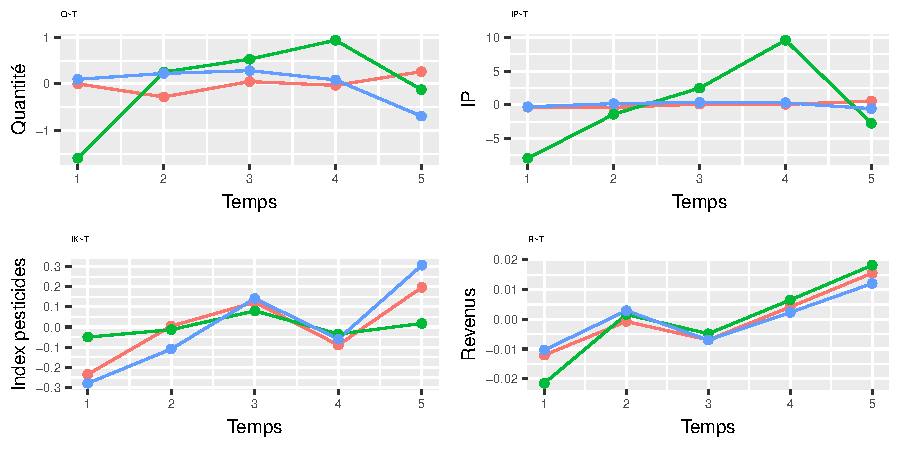
\includegraphics{note2pres_files/figure-latex/unnamed-chunk-90-1} 

}

\caption{Le comportement des résidus pour le modèle OLS}\label{fig:unnamed-chunk-90}
\end{figure}

\FloatBarrier

\hypertarget{d2.2-la-normalite-des-residus}{%
\paragraph{D2.2 La normalité des
résidus}\label{d2.2-la-normalite-des-residus}}

\FloatBarrier

\FloatBarrier

\begin{table}[!htbp] \centering 
  \caption{Shapiro-Wilk test de normalité des résidus, p-valeur} 
  \label{} 
\begin{tabular}{@{\extracolsep{5pt}} ccccccc} 
\\[-1.8ex]\hline 
\hline \\[-1.8ex] 
 & OLS c1 & IV-OLS c1 & OLS c2 & IV-OLS c2 & OLS c3 & IV-OLS c3 \\ 
\hline \\[-1.8ex] 
Equation d'offre & $0.00004$ & $0.0003$ & $0.014$ & $0.009$ & $0.00003$ & $0.044$ \\ 
\hline \\[-1.8ex] 
\end{tabular} 
\end{table}

\FloatBarrier

\newpage

\hypertarget{b2.3-diagnostiques-iv-ols}{%
\paragraph{B2.3 Diagnostiques IV-OLS}\label{b2.3-diagnostiques-iv-ols}}

\FloatBarrier

\begin{table}[!htbp] \centering 
  \caption{Diagnostiques d'estimateur IV, cluster 1} 
  \label{} 
\begin{tabular}{@{\extracolsep{5pt}} ccccc} 
\\[-1.8ex]\hline 
\hline \\[-1.8ex] 
 & df1 & df2 & statistic & p-value \\ 
\hline \\[-1.8ex] 
Weak instruments & $2$ & $141$ & $8.980$ & $0.0002$ \\ 
Wu-Hausman & $1$ & $141$ & $23.590$ & $0.00000$ \\ 
\hline \\[-1.8ex] 
\end{tabular} 
\end{table}

\FloatBarrier

\FloatBarrier

\begin{table}[!htbp] \centering 
  \caption{Diagnostiques d'estimateur IV, cluster 2} 
  \label{} 
\begin{tabular}{@{\extracolsep{5pt}} ccccc} 
\\[-1.8ex]\hline 
\hline \\[-1.8ex] 
 & df1 & df2 & statistic & p-value \\ 
\hline \\[-1.8ex] 
Weak instruments & $2$ & $1$ & $51.783$ & $0.098$ \\ 
Wu-Hausman & $1$ & $1$ & $1,511,030,356,715,090,395,088,268,284,282$ & $0$ \\ 
\hline \\[-1.8ex] 
\end{tabular} 
\end{table}

\FloatBarrier

\FloatBarrier

\begin{table}[!htbp] \centering 
  \caption{Diagnostiques d'estimateur IV, cluster 3} 
  \label{} 
\begin{tabular}{@{\extracolsep{5pt}} ccccc} 
\\[-1.8ex]\hline 
\hline \\[-1.8ex] 
 & df1 & df2 & statistic & p-value \\ 
\hline \\[-1.8ex] 
Weak instruments & $2$ & $191$ & $0.322$ & $0.725$ \\ 
Wu-Hausman & $1$ & $191$ & $58.351$ & $0$ \\ 
\hline \\[-1.8ex] 
\end{tabular} 
\end{table}

\FloatBarrier

\newpage

\hypertarget{d3-analyse-des-resultats-m2}{%
\subsubsection{D3 Analyse des résultats
M2}\label{d3-analyse-des-resultats-m2}}

\hypertarget{d3.1-independance-des-residus}{%
\paragraph{D3.1 Independance des
résidus}\label{d3.1-independance-des-residus}}

\FloatBarrier

\begin{figure}[!htbp]

{\centering \includegraphics{note2pres_files/figure-latex/unnamed-chunk-99-1} 

}

\caption{Les résidus contre la variable prédite, le cadre SUR}\label{fig:unnamed-chunk-99}
\end{figure}

\FloatBarrier

\newpage

\hypertarget{d3.2-la-normalite-des-residus-le-cadre-de-sur}{%
\subsubsection{D3.2 La normalité des résidus, le cadre de
SUR}\label{d3.2-la-normalite-des-residus-le-cadre-de-sur}}

\FloatBarrier

\FloatBarrier

\begin{table}[!htbp] \centering 
  \caption{Shapiro-Wilk test de normalité, p-valeur} 
  \label{} 
\begin{tabular}{@{\extracolsep{5pt}} cccc} 
\\[-1.8ex]\hline 
\hline \\[-1.8ex] 
 & Cluster 1 & Cluster 2 & Cluster 3 \\ 
\hline \\[-1.8ex] 
Equation de demande & $0.00004$ & $0.115$ & $0.00003$ \\ 
Equation d'offre & $0.0001$ & $0.190$ & $0.0001$ \\ 
\hline \\[-1.8ex] 
\end{tabular} 
\end{table}

\FloatBarrier

\FloatBarrier

\begin{figure}[!htbp]

{\centering 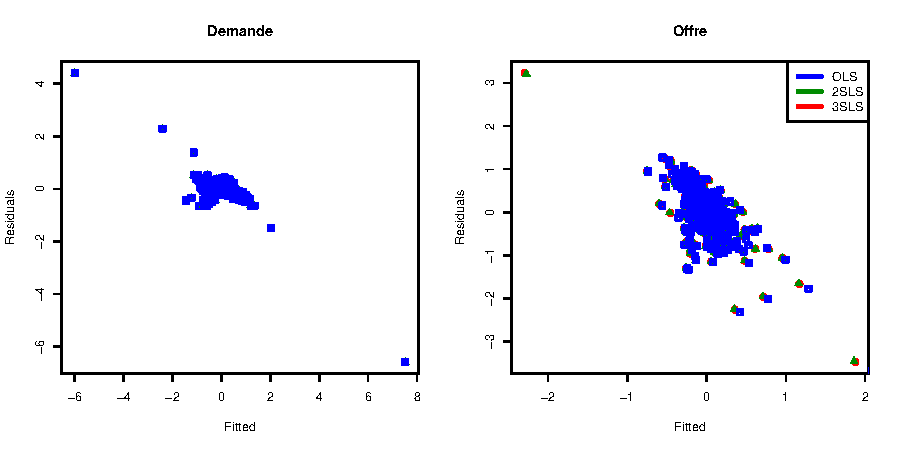
\includegraphics{note2pres_files/figure-latex/unnamed-chunk-102-1} 

}

\caption{Les PDF des résidus}\label{fig:unnamed-chunk-102}
\end{figure}

\FloatBarrier

\newpage

\hypertarget{references}{%
\section*{References}\label{references}}
\addcontentsline{toc}{section}{References}

\hypertarget{refs}{}
\leavevmode\hypertarget{ref-anderson2011global}{}%
Anderson, Kym, Signe Nelgen, and others. 2011. \emph{Global Wine
Markets, 1961 to 2009: A Statistical Compendium}. University of Adelaide
Press.

\leavevmode\hypertarget{ref-Butault2011}{}%
Butault Jean-Pierre, Jacquet Florence, Delame Nathalie, and Zardet
Guillaume. 2011. ``L'utilisation Des Pesticides En France : État Des
Lieux et Perspectives de Réduction.'' \emph{Note et études
Socio-économiques}, no. 35: 7--26.

\leavevmode\hypertarget{ref-cembalo2014}{}%
Cembalo, Luigi, Francesco Caracciolo, and Eugenio Pomarici. 2014.
``Drinking Cheaply: The Demand for Basic Wine in Italy.''
\emph{Australian Journal of Agricultural and Resource Economics} 58 (3):
374--91.

\leavevmode\hypertarget{ref-ineris}{}%
``Données de Vente de Pesticides Par Département.'' n.d. \emph{INERIS}.
\url{https://www.data.gouv.fr/fr/datasets/donnees-de-vente-de-pesticides-par-departement/\#_}.

\leavevmode\hypertarget{ref-Moghaddam2019}{}%
Fiona, Moghaddam, and Van Mastrigt Roméo. 2019. ``Comment L'utilisation
Des Pesticides N'a Cessé d'évoluer Ces 10 Dernières Années.''
\url{'https://www.franceculture.fr/ecologie-et-environnement/comment-lutilisation-de-pesticides-na-cesse-devoluer-ces-dix-dernieres-annees'}.

\leavevmode\hypertarget{ref-FranceAgriMer2011}{}%
FranceAgriMer. 2011. ``Note de Conjoncture.''
\url{'https://www.franceagrimer.fr/filieres-Vin-et-cidre/Vin/En-un-clic/Dossiers-des-Conseils-et-comites?moteur\%5BfiltreFiliere\%5D=1506\&moteur\%5BfiltreTypeContenu\%5D=analyse\&page=6'}.

\leavevmode\hypertarget{ref-hausman1996valuation}{}%
Hausman, Jerry A. 1996. ``Valuation of New Goods Under Perfect and
Imperfect Competition.'' In \emph{The Economics of New Goods}, 207--48.
University of Chicago Press.

\leavevmode\hypertarget{ref-franceagrimer}{}%
``Historique Des Prix Moyens Vrac Vsig et Igp.'' n.d.
\emph{FranceAgriMer}.
\url{http://visionet.franceagrimer.fr/Pages/OpenDocument.aspx?fileurl=SeriesChronologiques/productions\%20végétales/vin\%20et\%20cidriculture/prix\%20moyens/prix\%20moyens\%20vrac\%20VSIG\%20et\%20IGP/COT-VIN-HISTORIQUE_ACTVITE_PRIX_DEPUIS2000-C15-16.xls\&telechargersanscomptage=oui}.

\leavevmode\hypertarget{ref-Ifop2017}{}%
Ifop. 2017. ``Les Français, La Consommation écoresponsable et La
Transition écologique.''
\url{'https://www.wwf.fr/sites/default/files/doc-2017-10/171010_sondage_wwf_ifop_agriculture\%202.pdf'}.

\leavevmode\hypertarget{ref-CNIV2018}{}%
Interprofessions des Vins â appellation d'origine et â indication
géographique, Comité National des. 2018. ``Chiffres Clés.''
\url{'https://www.intervin.fr/etudes-et-economie-de-la-filiere/chiffres-cles'}.

\leavevmode\hypertarget{ref-Pujol2017}{}%
Jérome, Pujol. 2017. ``Apports de Produits Phytosanitaires En
Viticulture et Climat : Une Analyse â Partir Des Enquêtes Pratiques
Culturales.'' \emph{Agreste Les Dossiers}, no. 39: 3--25.

\leavevmode\hypertarget{ref-kremer2004}{}%
KREMER, Florence, and Catherine VIOT. 2004. ``Conflit et Coopération Au
Sein Du Canal: L'interaction Stratégique Entre La Grande Distribution et
Les Producteurs de La Filière Viti-Vinicole.''

\leavevmode\hypertarget{ref-laporte1996}{}%
Laporte, Catherine, and Marie-Claude PICHERY. 1996. ``Production costs
of AOC Burgundy wines.'' Research Report. Laboratoire d'analyse et de
techniques économiques(LATEC).
\url{https://hal.archives-ouvertes.fr/hal-01526958}.

\leavevmode\hypertarget{ref-mackay2018}{}%
MacKay, Alexander, and Nathan H Miller. 2018. ``Estimating Models of
Supply and Demand: Instruments and Covariance Restrictions.''

\leavevmode\hypertarget{ref-makela2006}{}%
MÄKELÄ, PIA, GERHARD GMEL, ULRIKE GRITTNER, HERVÉ KUENDIG, SANDRA
KUNTSCHE, KIM BLOOMFIELD, and ROBIN ROOM. 2006. ``DRINKING PATTERNS AND
THEIR GENDER DIFFERENCES IN EUROPE.'' \emph{Alcohol and Alcoholism} 41
(October): i8--i18. \url{https://doi.org/10.1093/alcalc/agl071}.

\leavevmode\hypertarget{ref-outreville2010}{}%
Outreville, J François. 2010. ``Les Facteurs Déterminant Le Prix Du
Vin.'' \emph{Enometrica} 3 (1): 25--33.

\leavevmode\hypertarget{ref-insee}{}%
``Revenu et Pauvreté Des Ménages.'' 2016. \emph{INSEE}.
\url{https://www.insee.fr/fr/statistiques/4190004\#consulter}.

\leavevmode\hypertarget{ref-Prudent2018}{}%
Robin, Prudent. 2018. ``Enquête Franceinfo. Additifs, Pesticides... Le
Vin Que Vous Buvez Ne Contient Pas Que Du Raisin : Découvrez Le Résultat
de Nos Analyse.''
\url{'https://www.francetvinfo.fr/economie/emploi/metiers/agriculture/enquete-franceinfo-additifs-pesticides-le-vin-que-vous-buvez-ne-contient-pas-que-du-raisin-decouvrez-le-resultat-de-nos-analyses_2957897.html'}.

\leavevmode\hypertarget{ref-ssm}{}%
``Statistiques Viti-Vinicoles - Relevés Annuels Des Stocks et Des
Récoltes Depuis 2009.'' n.d. \emph{SSM Finances Publiques}.
\url{https://www.data.gouv.fr/fr/datasets/statistiques-viti-vinicoles-releves-annuels-des-stocks-et-des-recoltes-depuis-2009/}.

\leavevmode\hypertarget{ref-steiner2004}{}%
Steiner, Bodo. 2004. ``French Wines on the Decline? Econometric Evidence
from Britain.'' \emph{Journal of Agricultural Economics} 55 (2):
267--88.

\leavevmode\hypertarget{ref-wooldridge2005instrumental}{}%
Wooldridge, Jeffrey M. 2005. ``Instrumental Variables Estimation with
Panel Data.'' \emph{Econometric Theory} 21 (4): 865--69.


\end{document}
